% Copyright (c) 2008-2009 solvethis
% Copyright (c) 2010-2011 Casper Ti. Vector
% Public domain.

\chapter{数值算例与结论分析}
    \indent 本章我们将用前面所得的分区计算积分核的算法来进行破裂数值模拟。旨在通过分区处理积分核的计算方法与原有计算方法的对比,突出分区计算法在计算破裂过程中的高效性。同时,我们将对结果进行分析。所有程序在~Lunix~服务器上运行,服务器内存~125.5G,CPU~为~Intel(R) Xeon(R) CPU E7-4809 v3 @ 2.00GHz。
	\section{数值算例}
    \indent 我们将通过具体的数值算例来模拟破裂过程,以达到检验本文分区计算积分核的算法的有效性。使用边界积分方程模拟破裂演化过程,大体可以分为三个步骤:网格离散,离散化积分核积分,破裂的时间演进模拟。而分区计算法优化的便是离散化积分核积分这个部分,该算法能够大大的减小了计算积分核的时间。

		\subsection{数值算例一}
    \indent 首先我们研究一个尺度适中的平面问题。研究断层为一矩形断层面,长为~2.7km,宽为~1.6km,每个三角形网格的边长为~0.1km,如图~\ref{fig:rupture-model1}~所示。
 \begin{figure}[H]
    \centerin
   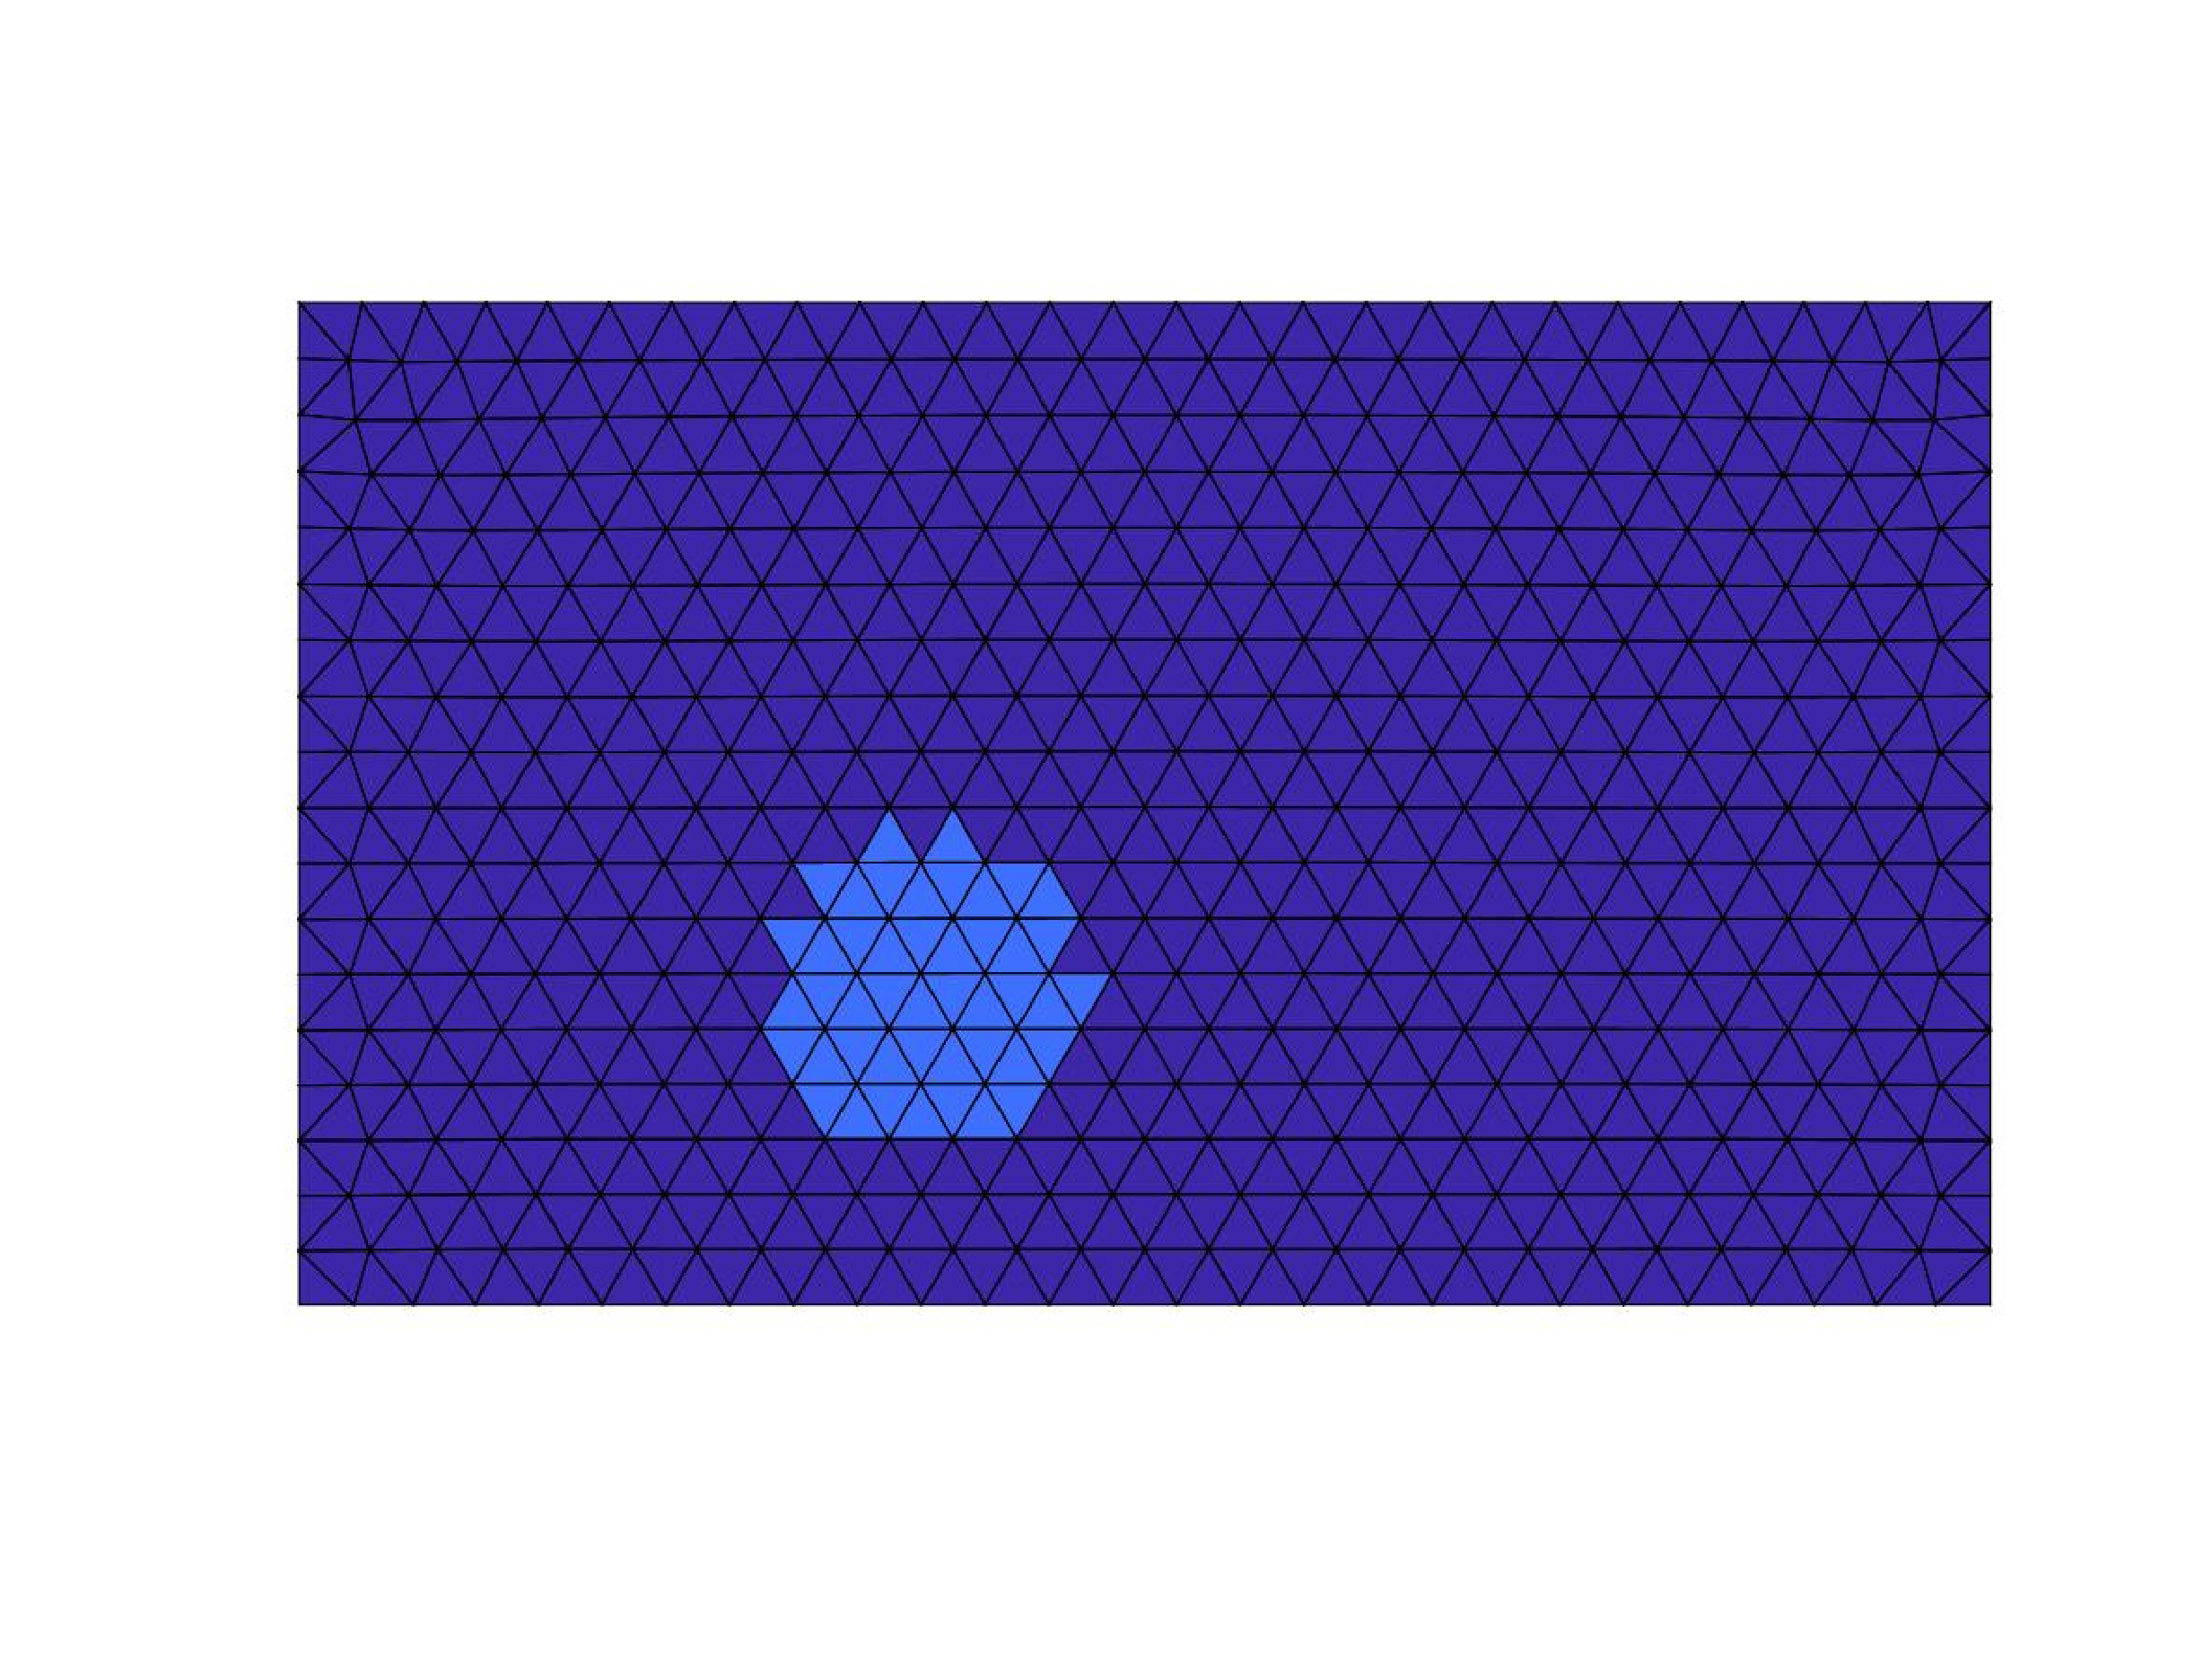
\includegraphics[trim = 0mm 40mm 80mm 40mm, clip=true,width=0.8\linewidth]{img/ruptuerprocess_step1.eps}
    \caption{ 平面断层模型(图中浅色区为初始破裂)} \label{fig:rupture-model1}
  \end{figure}
    \noindent 一共有~958~个单元,525~个点。初始的破裂区为以网格坐标(0.25,1)为中心,半径为0.25公里的圆形区域~(如图~\ref{fig:rupture-model1}~中浅色区所示)。P~波数波速为~5.6km/s~,S波波速为~3.23km/s。断层的初始应力分布为:圆形区域的初始应力大于破裂强度,大小为~$\sigma_{0} = 1.2 T_0$,圆形以外的区域初始应力小于破裂强度,大小为~$\sigma_{0}=0.8T_{0}$~。 在该初始应力条件下,该平面断层为以中间圆为初始破裂区域进行自发破裂过程。一共计算~150~个时间步。我们分别采用两种方法来计算积分核值。可以得到,用原有方法计算积分核需要~936.98s。 而我们采用分区处理的办法,计算积分核 只需要~269.5s,效率提高了~71.2\%。最后,将由分区法所得的积分核用以破裂过程的计算,可以得到破裂图像如图~\ref{fig:rupture-process}~所示。可见,在保证正确性的条件下,分区计算积分核 的方法具有更高的效率。
    
\begin{figure}[!h]
  \centerin
  \includegraphics[width=0.99\linewidth]{img/rupture1.png}
    \caption{ 平面断层破裂过程} \label{fig:rupture-process}
 \end{figure}
  
    \begin{comment}
    \begin{figure}[!h]
  \centering
  \begin{subfigure}[b]{0.3\linewidth}
    \includegraphics[trim = 20mm 30mm 20mm 30mm,clip=true,width=\linewidth]{img/ruptuerprocess_step3.jpg}
    %\label{a}
  \end{subfigure}
  \begin{subfigure}[b]{0.3\linewidth}
    \includegraphics[trim = 20mm 30mm 20mm 30mm,clip=true,width=\linewidth]{img/ruptuerprocess_step10.jpg}
  \end{subfigure}
  \begin{subfigure}[b]{0.3\linewidth}
    \includegraphics[trim = 20mm 30mm 20mm 30mm,clip=true,width=\linewidth]{img/ruptuerprocess_step20.jpg}
  \end{subfigure}
  \begin{subfigure}[b]{0.3\linewidth}
    \includegraphics[trim = 20mm 30mm 20mm 30mm,clip=true,width=\linewidth]{img/ruptuerprocess_step30.jpg}
  \end{subfigure}
  \begin{subfigure}[b]{0.3\linewidth}
    \includegraphics[trim = 20mm 30mm 20mm 30mm,clip=true,width=\linewidth]{img/ruptuerprocess_step35.jpg}
    %\label{a}
  \end{subfigure}
  \begin{subfigure}[b]{0.3\linewidth}
    \includegraphics[trim = 20mm 30mm 20mm 30mm,clip=true,width=\linewidth]{img/ruptuerprocess_step40.jpg}
  \end{subfigure}
  \begin{subfigure}[b]{0.3\linewidth}
    \includegraphics[trim = 20mm 30mm 20mm 30mm,clip=true,width=\linewidth]{img/ruptuerprocess_step50.jpg}

  \end{subfigure}
  \begin{subfigure}[b]{0.3\linewidth}
    \includegraphics[trim = 20mm 30mm 20mm 30mm,clip=true,width=\linewidth]{img/ruptuerprocess_step55.jpg}
  \end{subfigure}
  \begin{subfigure}[b]{0.3\linewidth}
    \includegraphics[trim = 20mm 30mm 20mm 30mm,clip=true,width=\linewidth]{img/ruptuerprocess_step60.jpg}
    %\label{a}
  \end{subfigure}
  \begin{subfigure}[b]{0.3\linewidth}
    \includegraphics[trim = 20mm 30mm 20mm 30mm,clip=true,width=\linewidth]{img/ruptuerprocess_step70.jpg}
  \end{subfigure}
  \begin{subfigure}[b]{0.3\linewidth}
    \includegraphics[trim = 20mm 30mm 20mm 30mm,clip=true,width=\linewidth]{img/ruptuerprocess_step80.jpg}
  \end{subfigure}
  \begin{subfigure}[b]{0.3\linewidth}
    \includegraphics[trim = 20mm 30mm 20mm 30mm,clip=true,width=\linewidth]{img/ruptuerprocess_step90.jpg}
  \end{subfigure}
  \caption{ 平面断层破裂过程66}
\end{figure}
\end{comment}
   
		\subsection{数值算例二}
    \indent 接着我们考虑一个复杂断层系统的情况。研究的断层为一弯折断层,如图~\ref{fig:rupture-model2}~所示。该弯折断层由三个平面构成,其中弯折的平面与水平面夹角为~$40.13^{\circ}$。该弯折断层离散为1073个单元,624个点。在弯折断层的第一个平面设置与数值算例一中平面断层上相同的圆形破裂区。
    
    \begin{figure}[H]
 \centerin
  \includegraphics[width=0.8\linewidth]{img/3Druptuerprocess_step1.png}
    \caption{ 弯折断层模型(图中浅色区为初始破裂区)} \label{fig:rupture-model2}
  \end{figure}
 \indent 一共计算~200~个时间步。同样的我们仍然采用两种计算方式计算积分核的值。若采用原方法需要~2298.41s才能计算得出结果,而采用分区计算积分核的方式,计算时长为~663.0s。计算效率提高了~71.14\%。利用计算所得的积分核可以得到破裂过程图如图~\ref{fig:3d-rupture}~所示。
 
 \begin{figure}[!h]
  \centerin
  \includegraphics[width=0.99\linewidth]{img/rupture2.png}
    \caption{ 弯折断层破裂过程} \label{fig:3d-rupture}
 \end{figure}
 
   \begin{comment}
    \begin{figure}[!h]
  \centering
    \begin{subfigure}[b]{0.45\linewidth}
    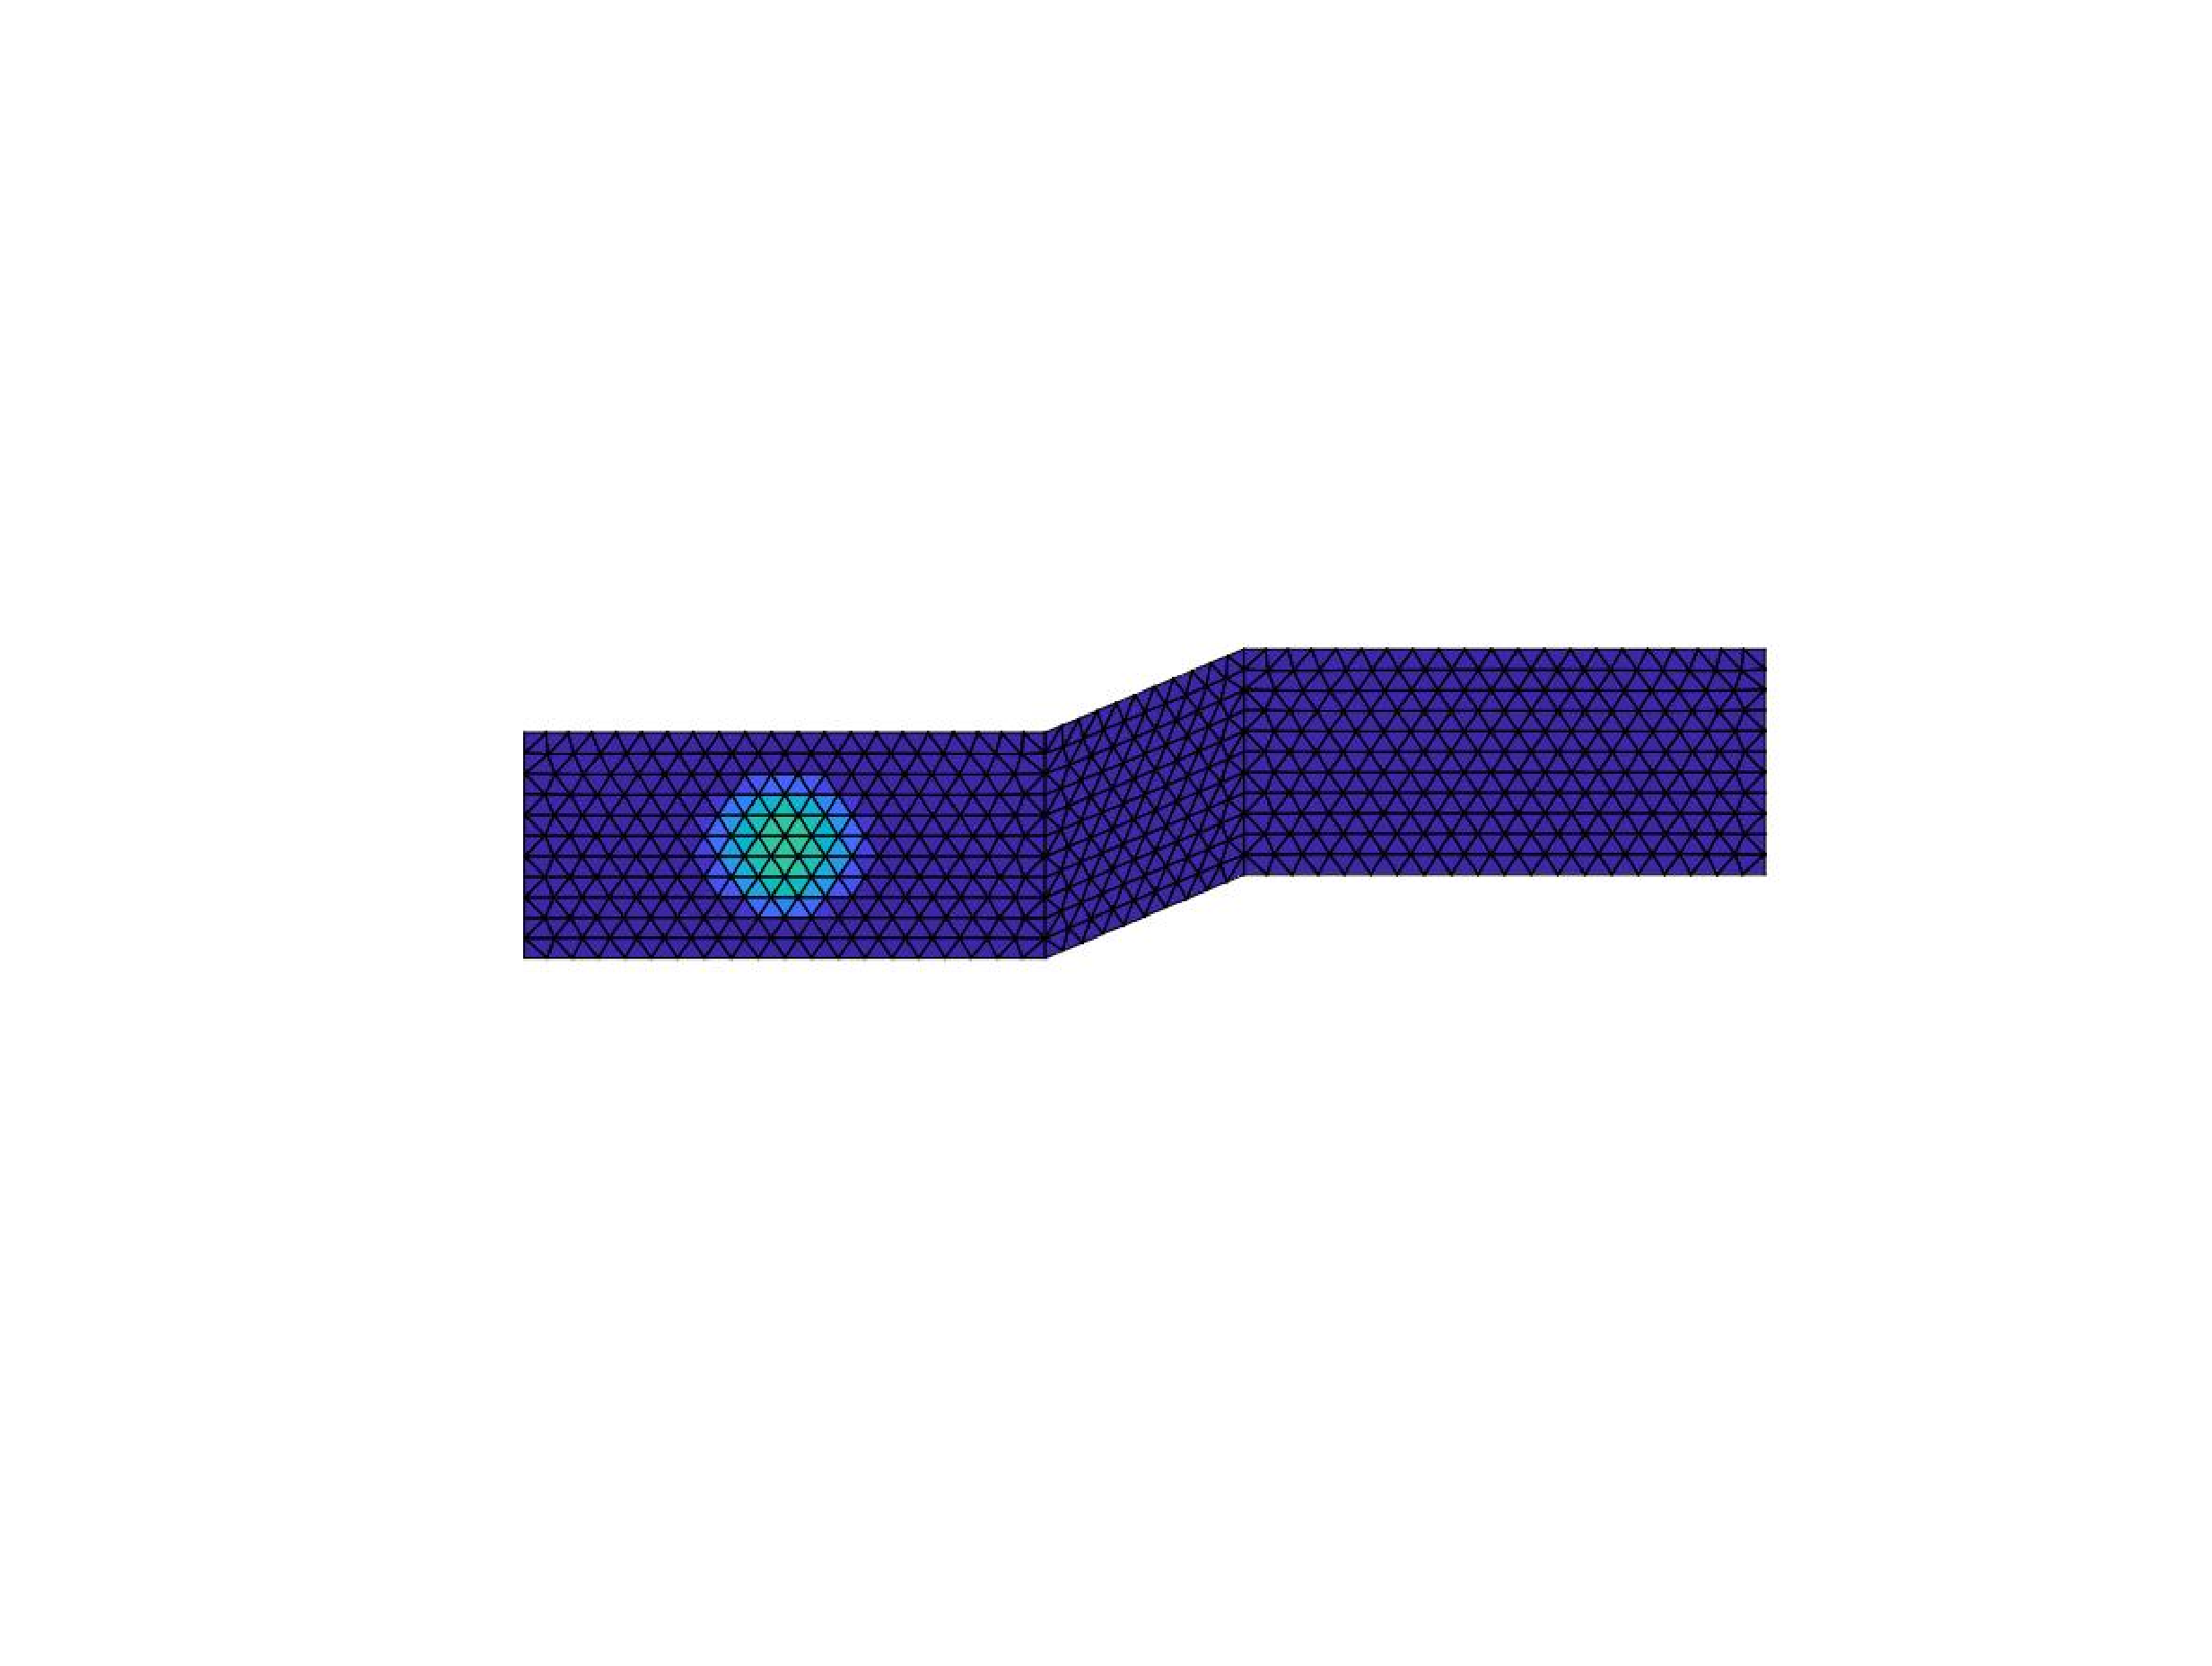
\includegraphics[trim = 100mm 120mm 100mm 120mm,clip=true, width=\linewidth]{img/3Druptuerprocess_step10.eps}
  \end{subfigure}
    \begin{subfigure}[b]{0.45\linewidth}
    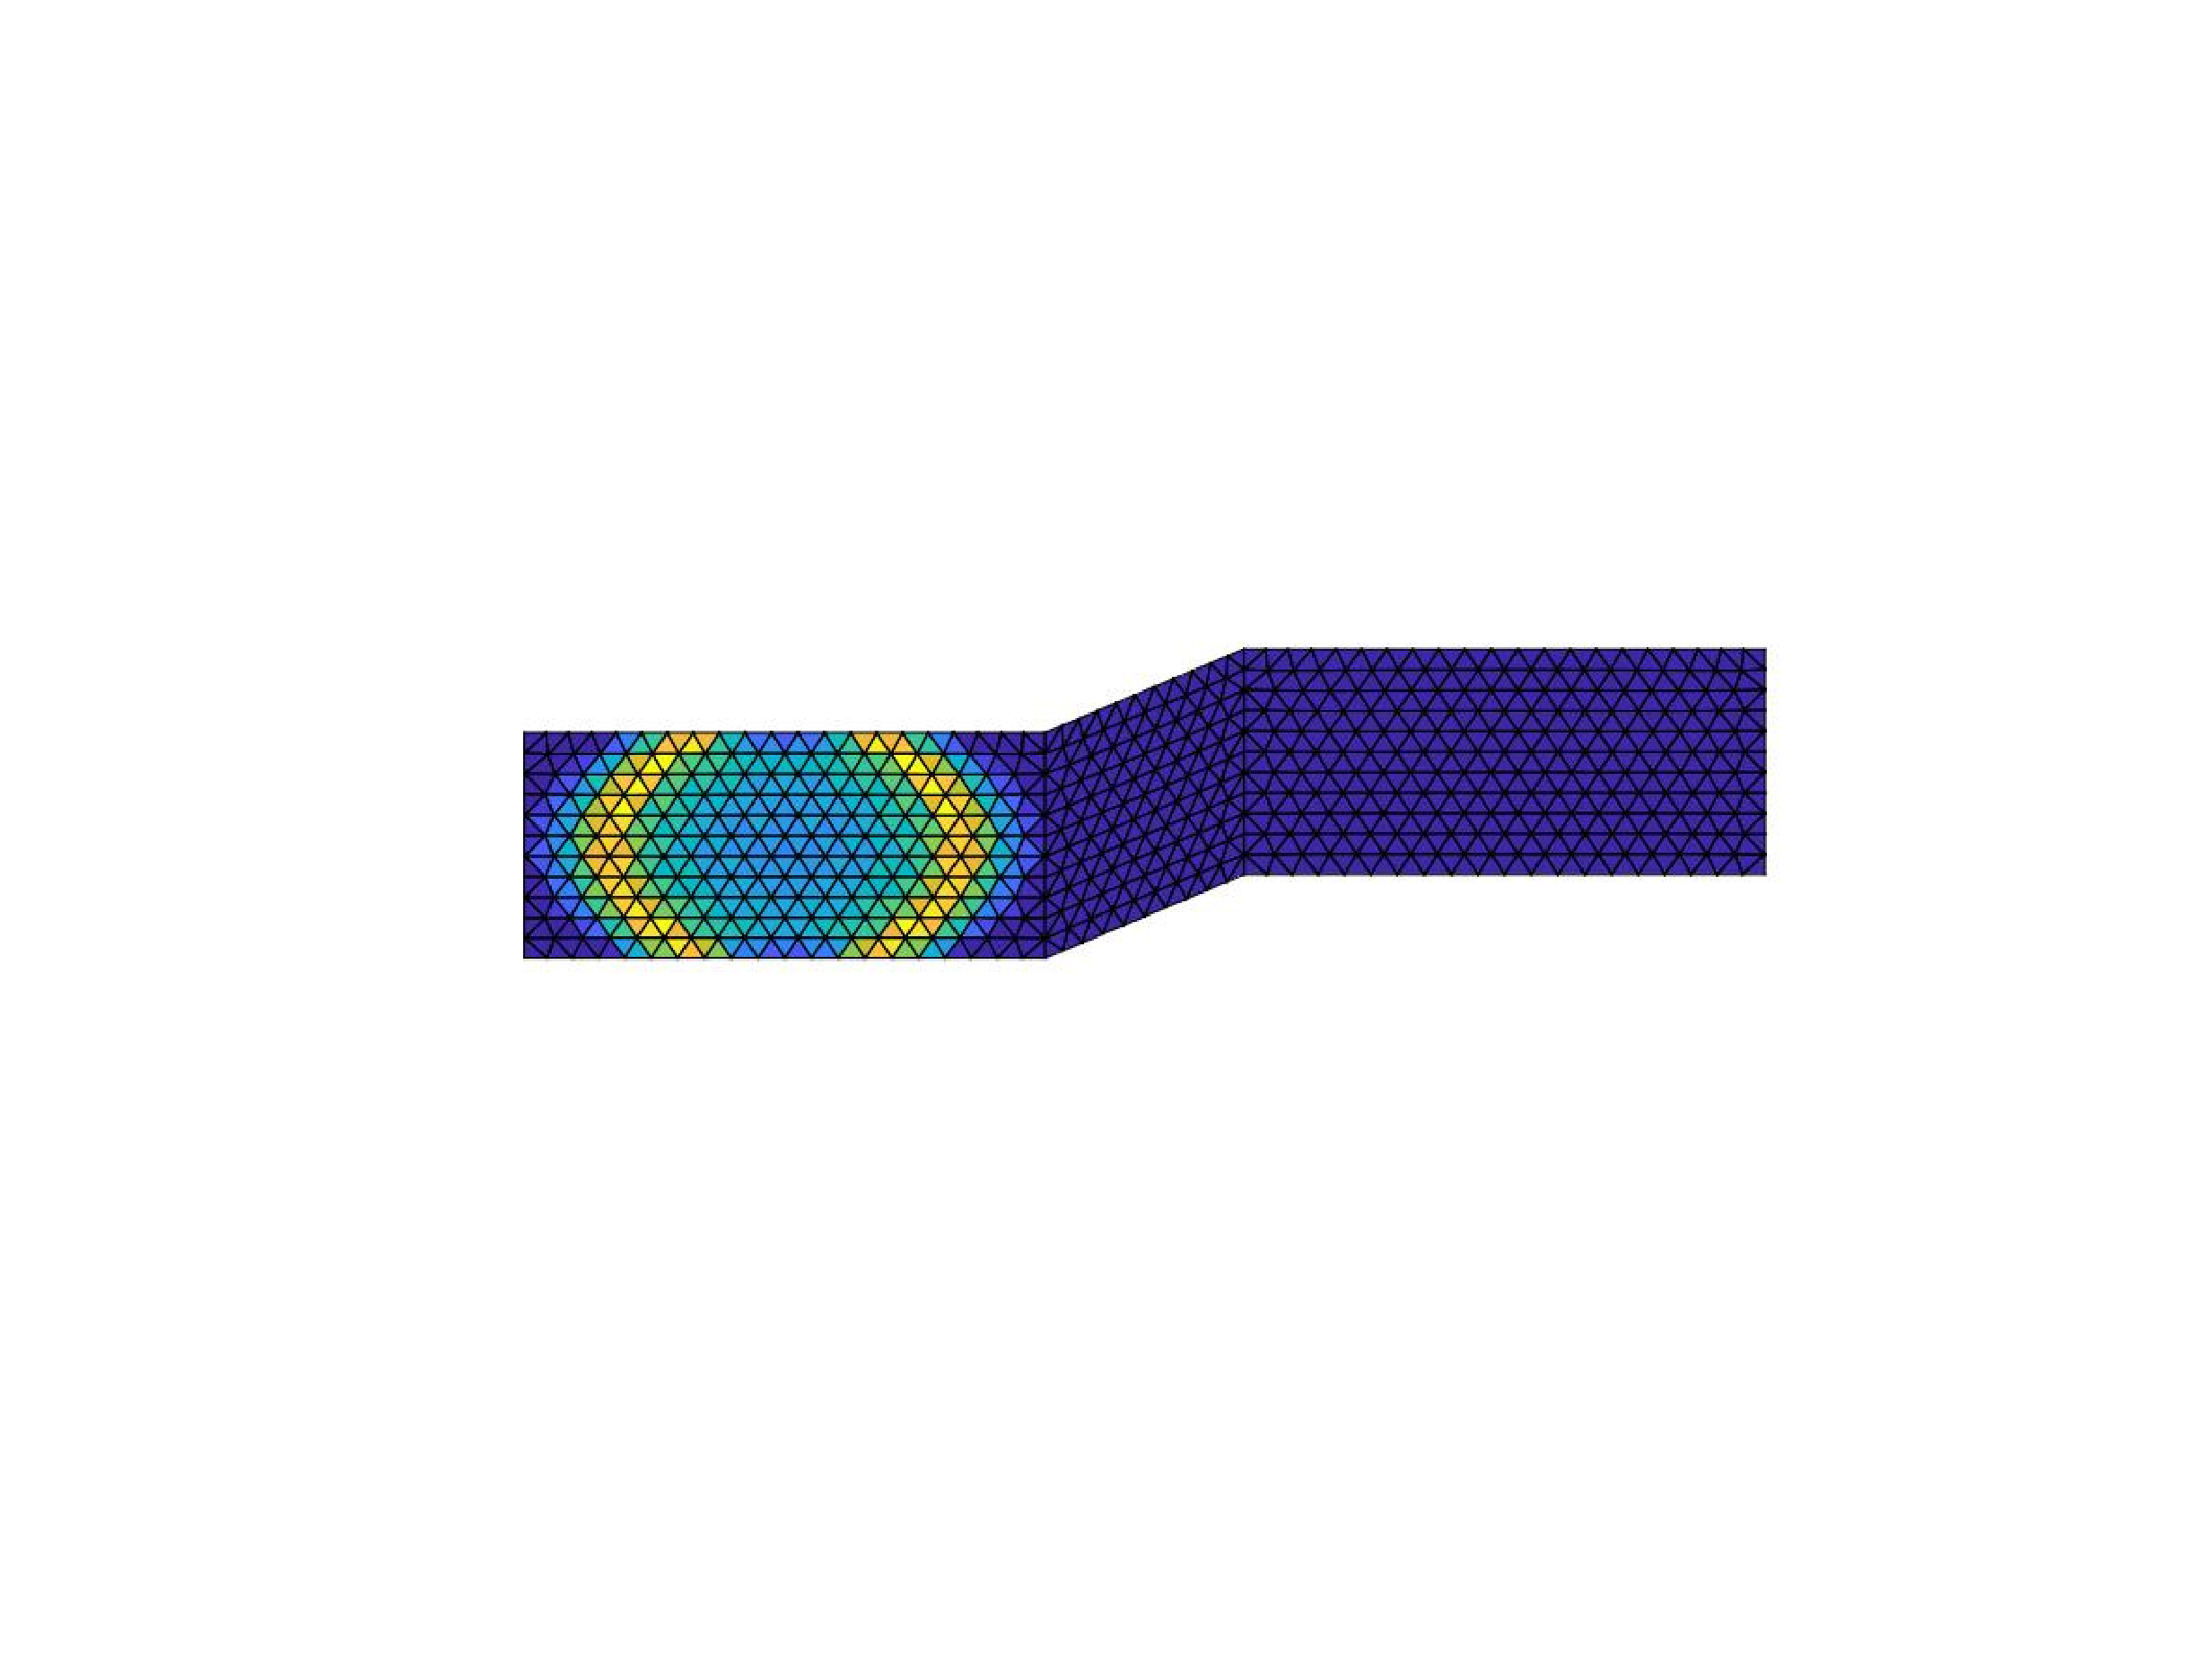
\includegraphics[trim = 100mm 120mm 100mm 120mm,clip=true, width=\linewidth]{img/3Druptuerprocess_step60.eps}
  \end{subfigure}
  
  \begin{subfigure}[b]{0.45\linewidth}
    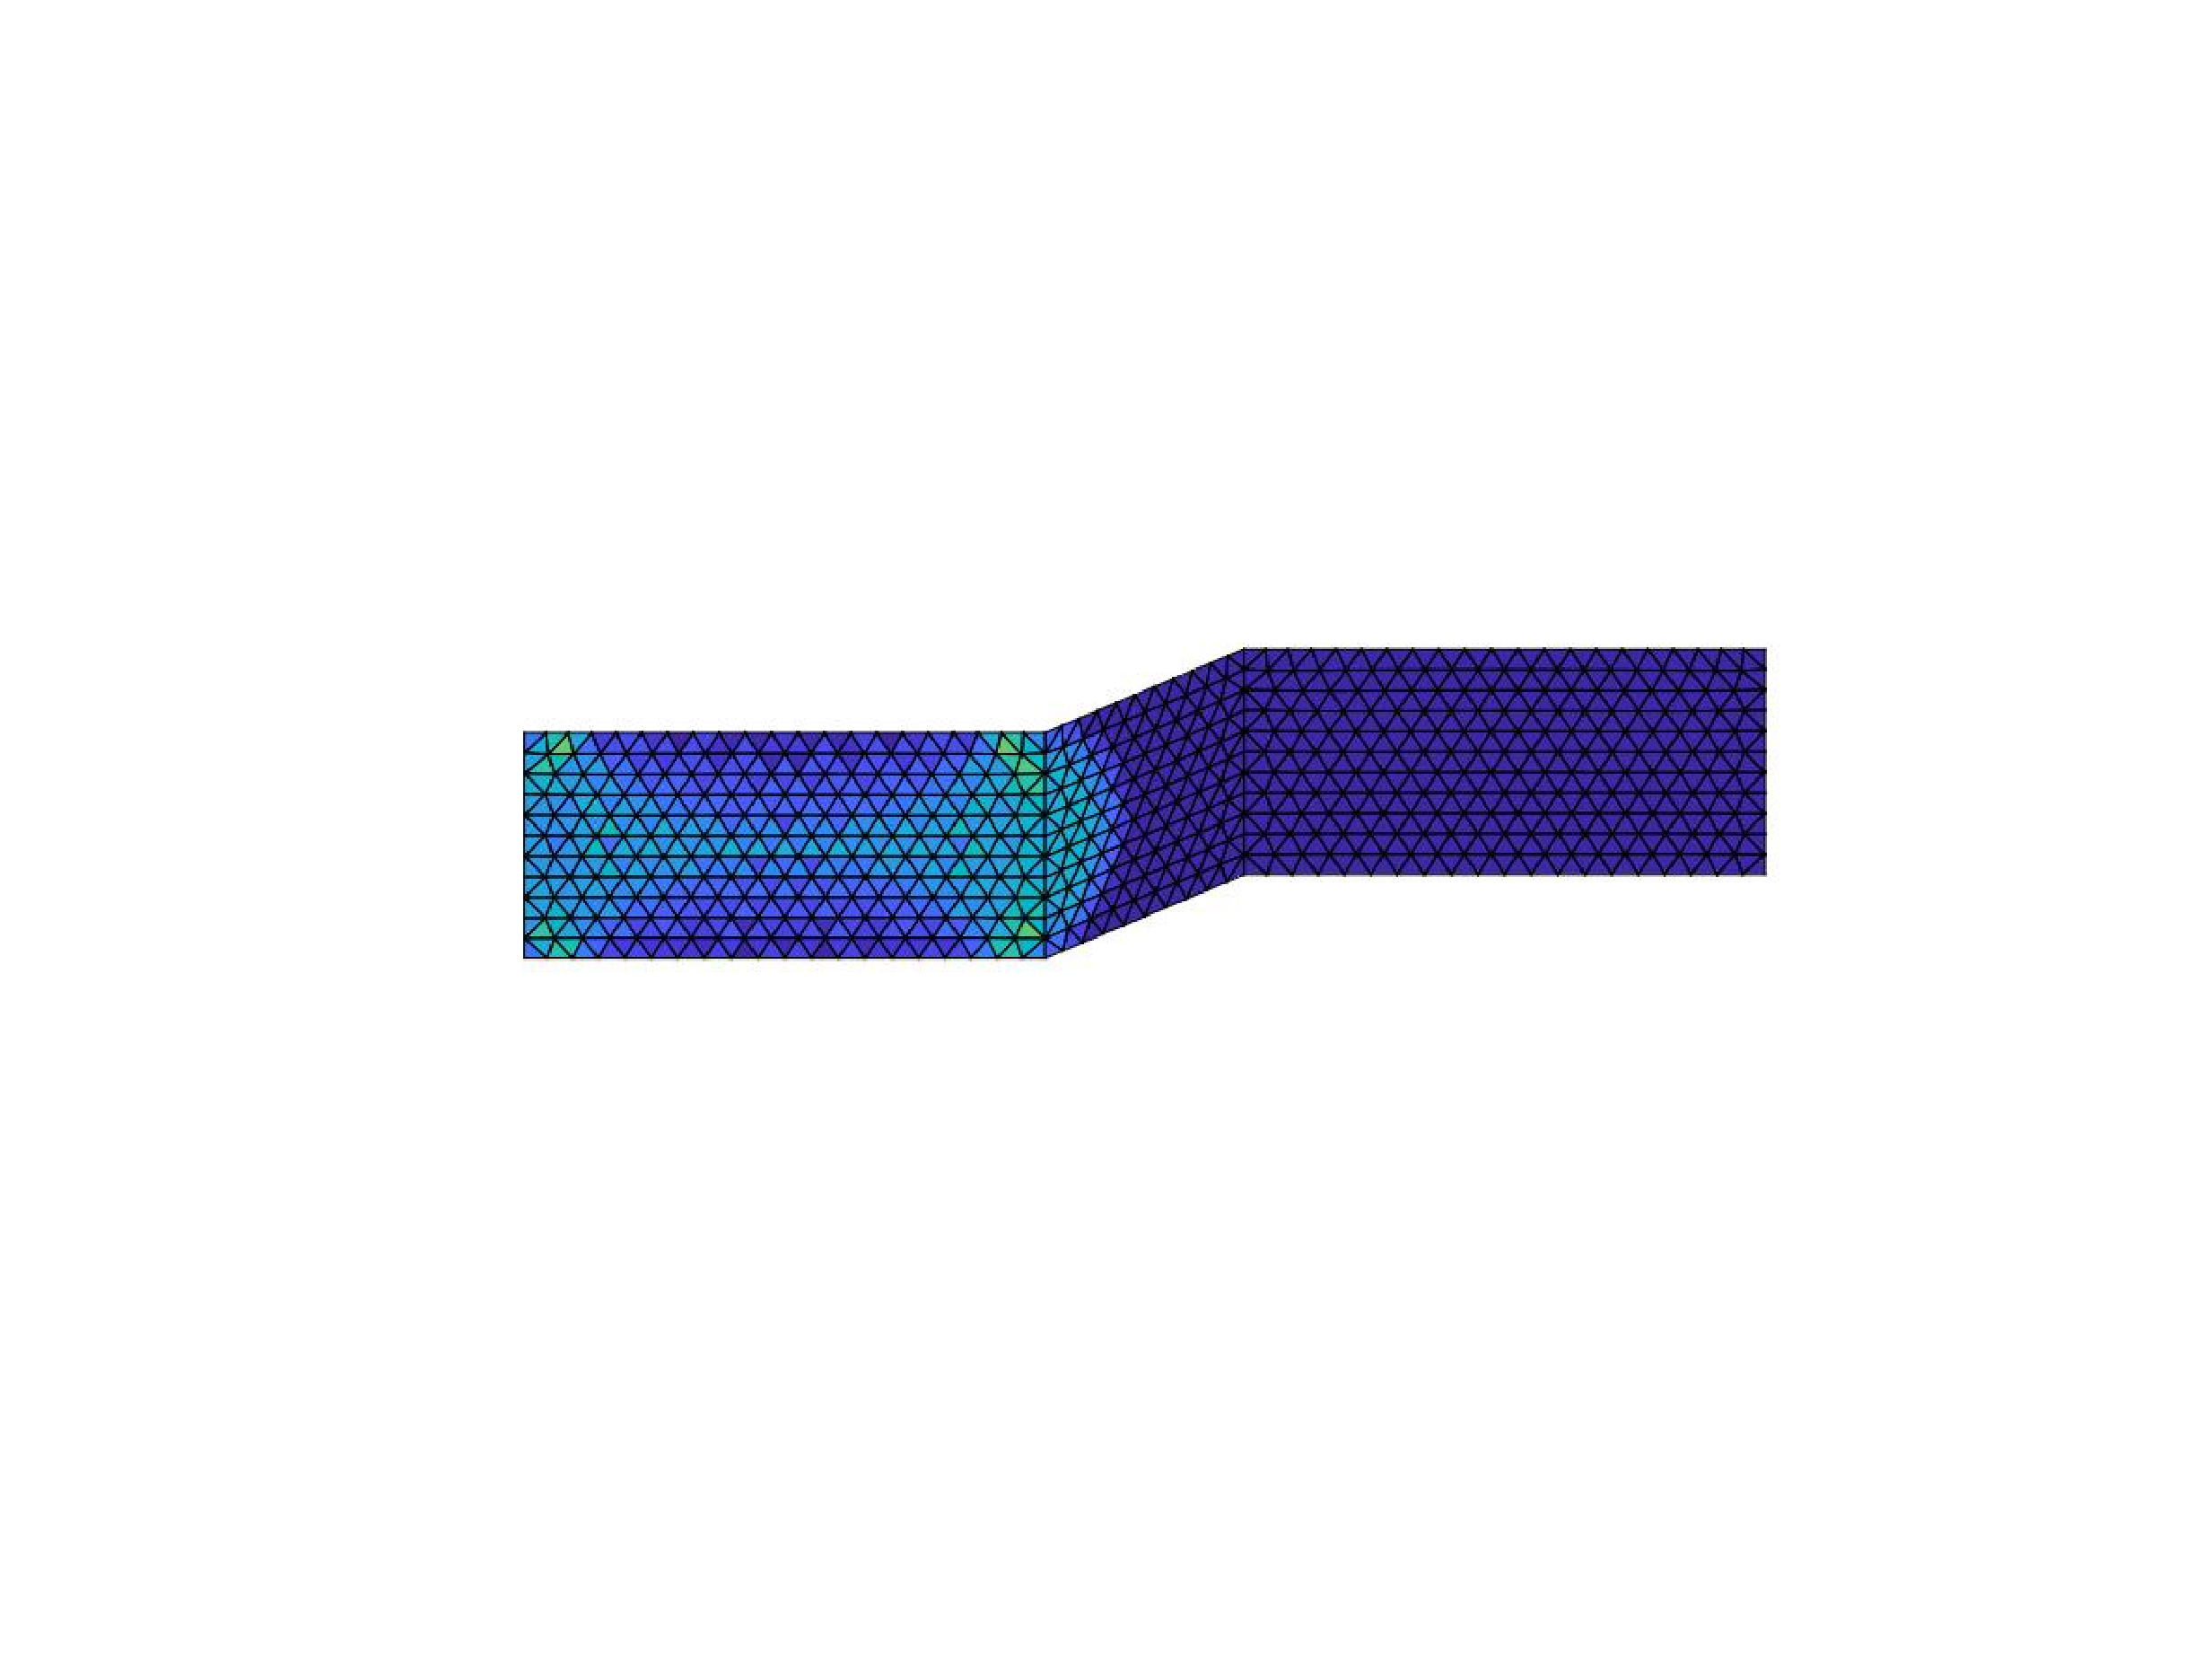
\includegraphics[trim = 100mm 120mm 100mm 120mm,clip=true, width=\linewidth]{img/3Druptuerprocess_step90.eps}
  \end{subfigure}
  \begin{subfigure}[b]{0.45\linewidth}
    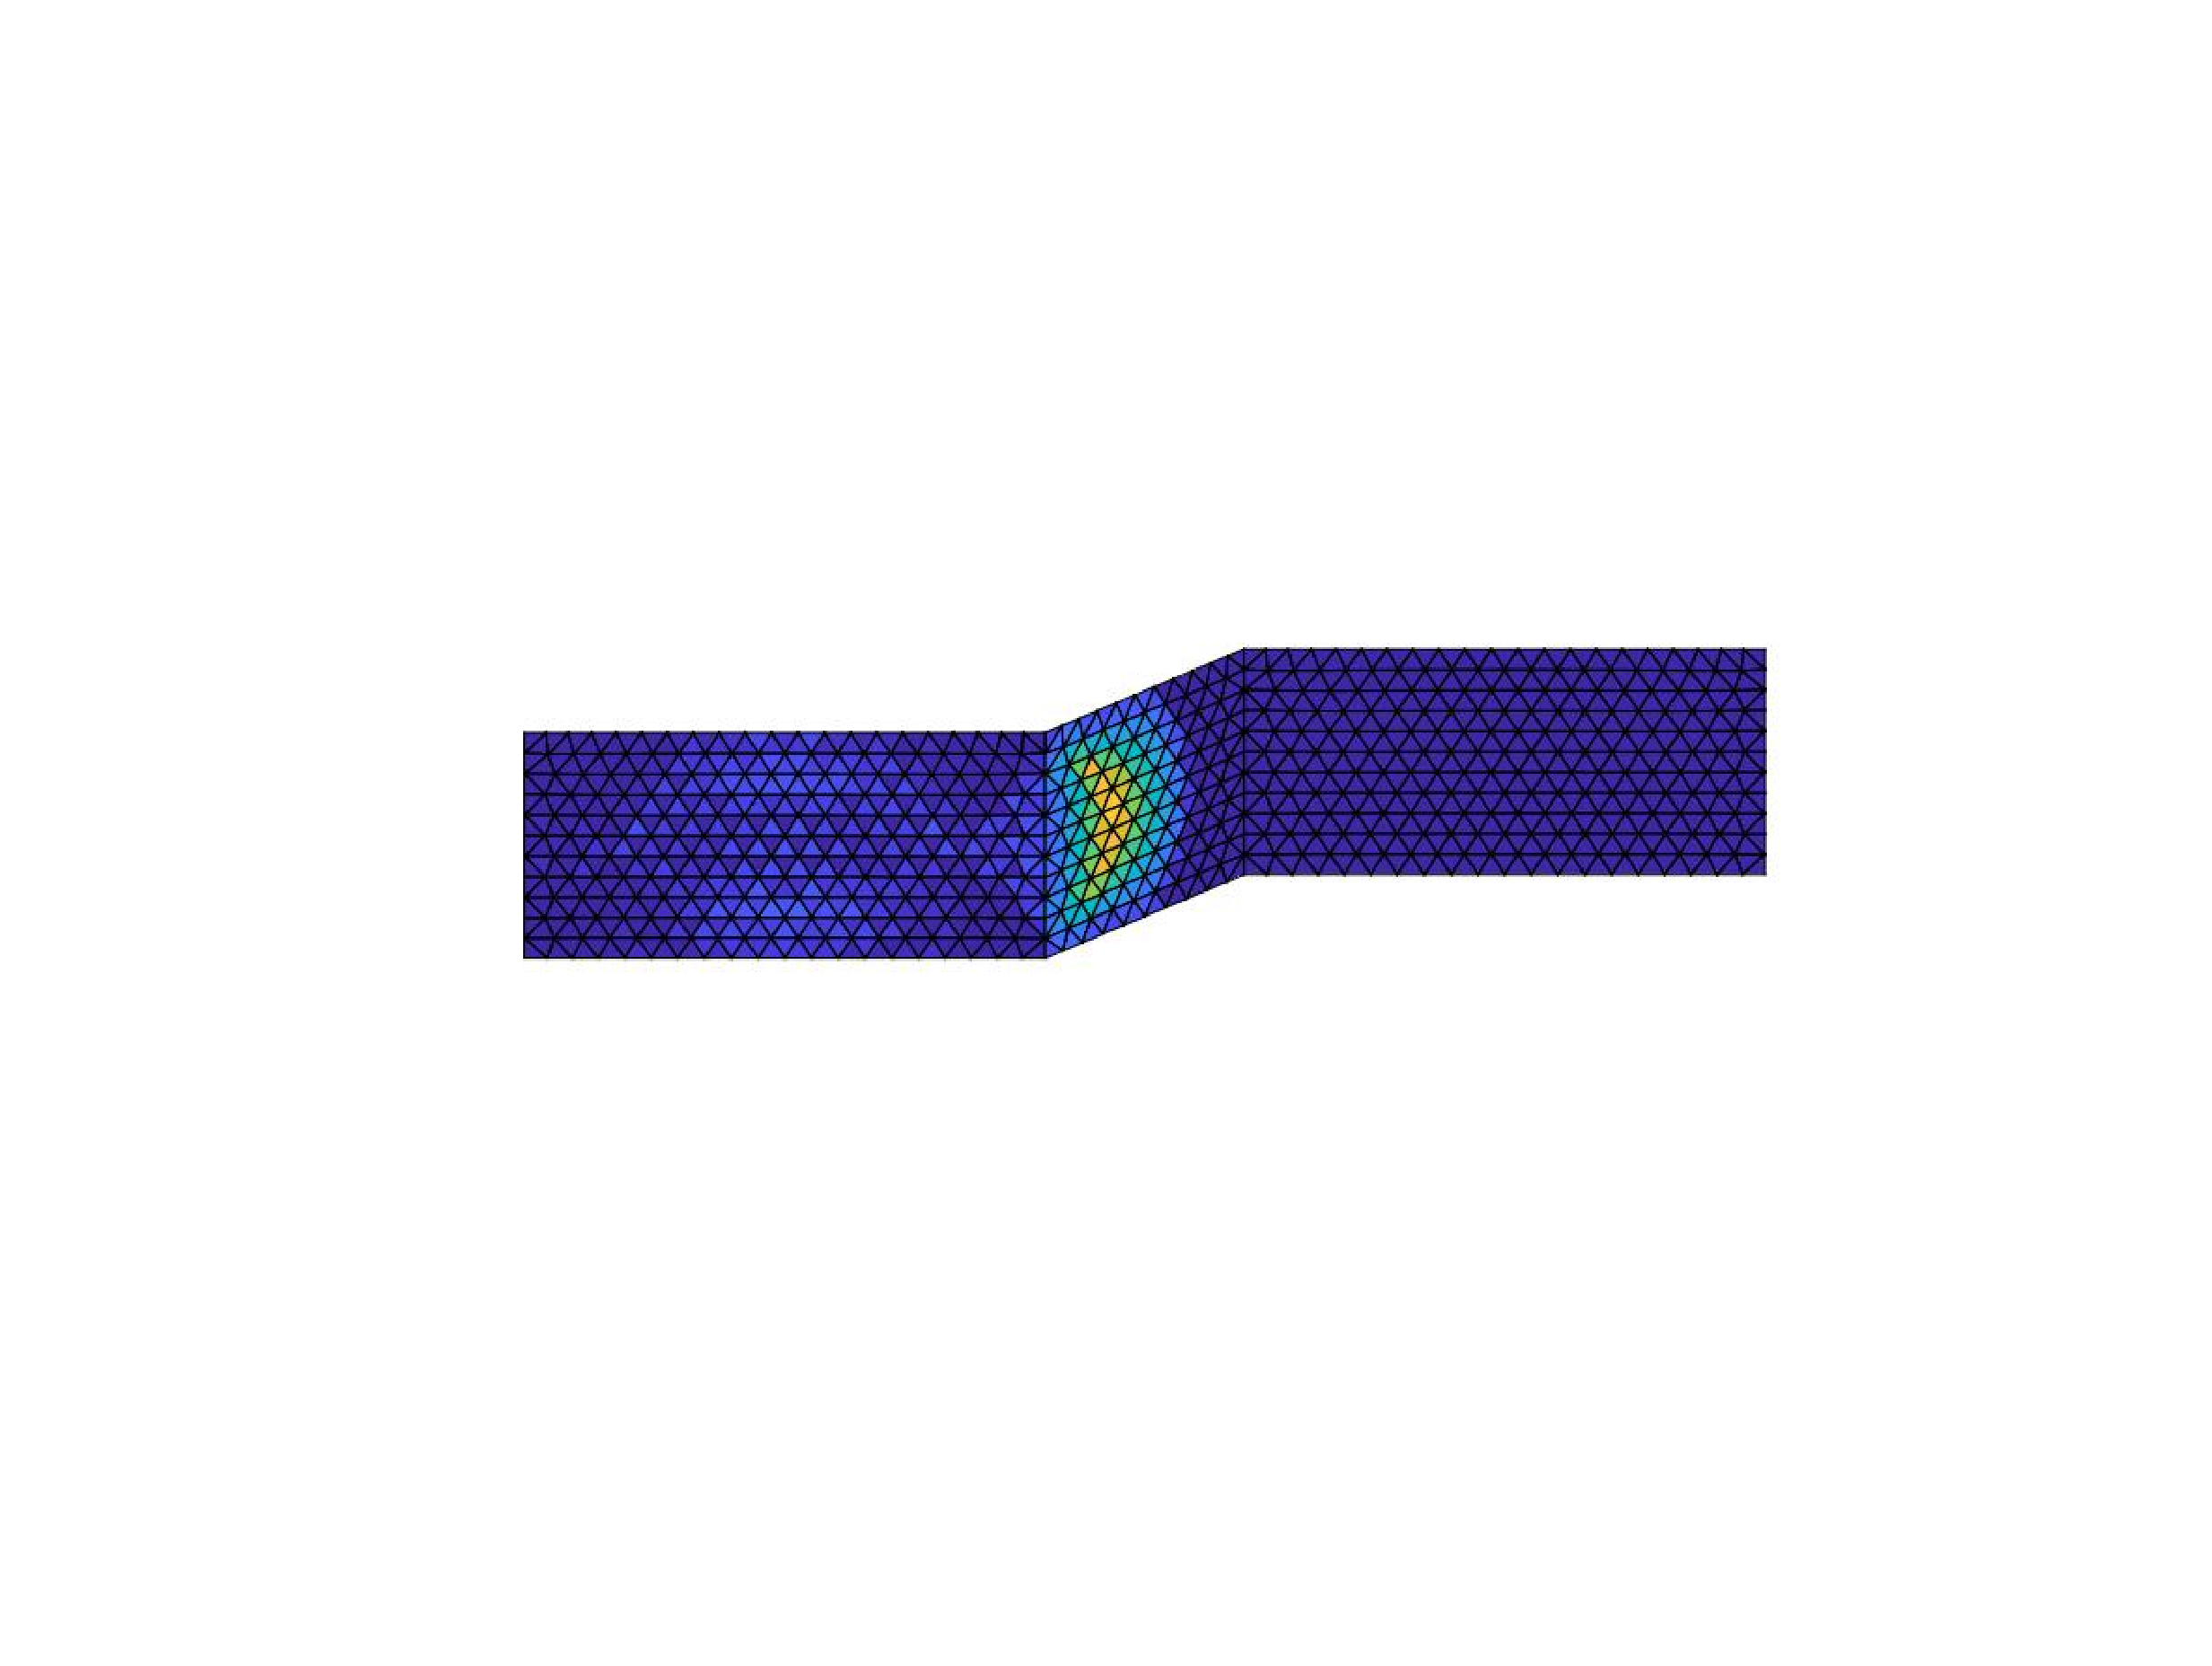
\includegraphics[trim = 100mm 120mm 100mm 120mm,clip=true, width=\linewidth]{img/3Druptuerprocess_step110.eps}
  \end{subfigure}
  
  \begin{subfigure}[b]{0.45\linewidth}
    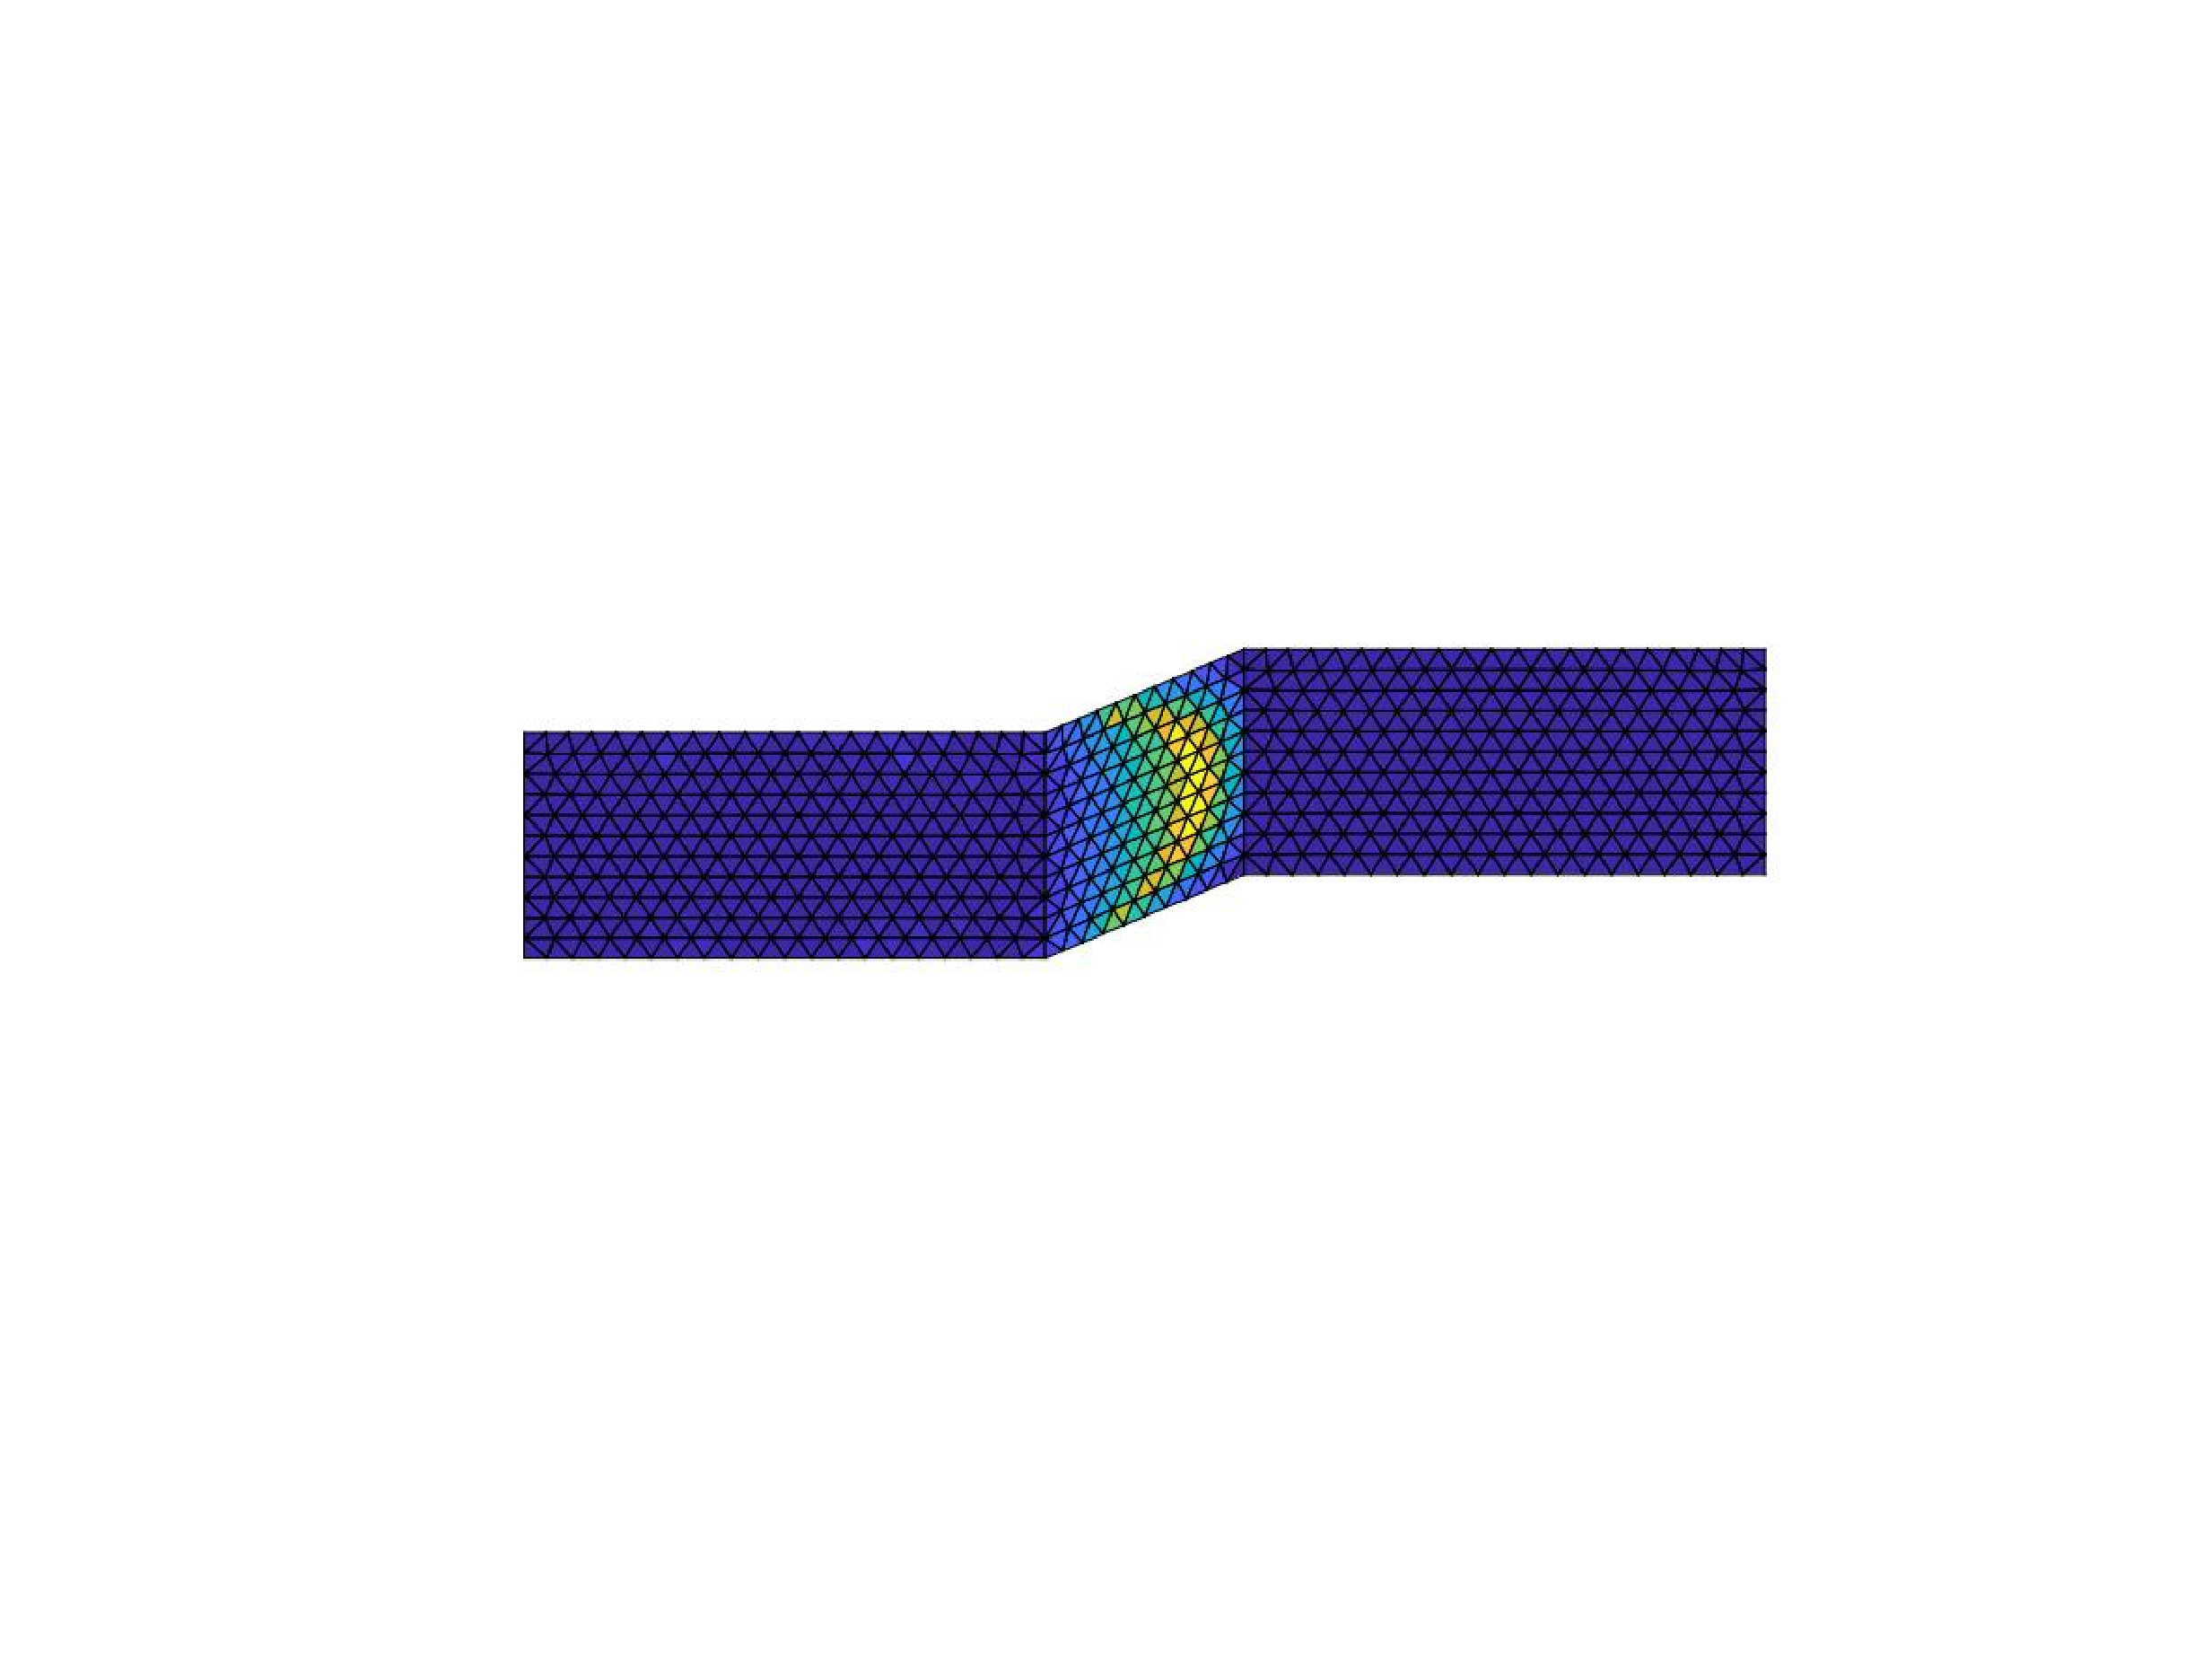
\includegraphics[trim = 100mm 120mm 100mm 120mm,clip=true, width=\linewidth]{img/3Druptuerprocess_step130.eps}
  \end{subfigure}
  \begin{subfigure}[b]{0.45\linewidth}
    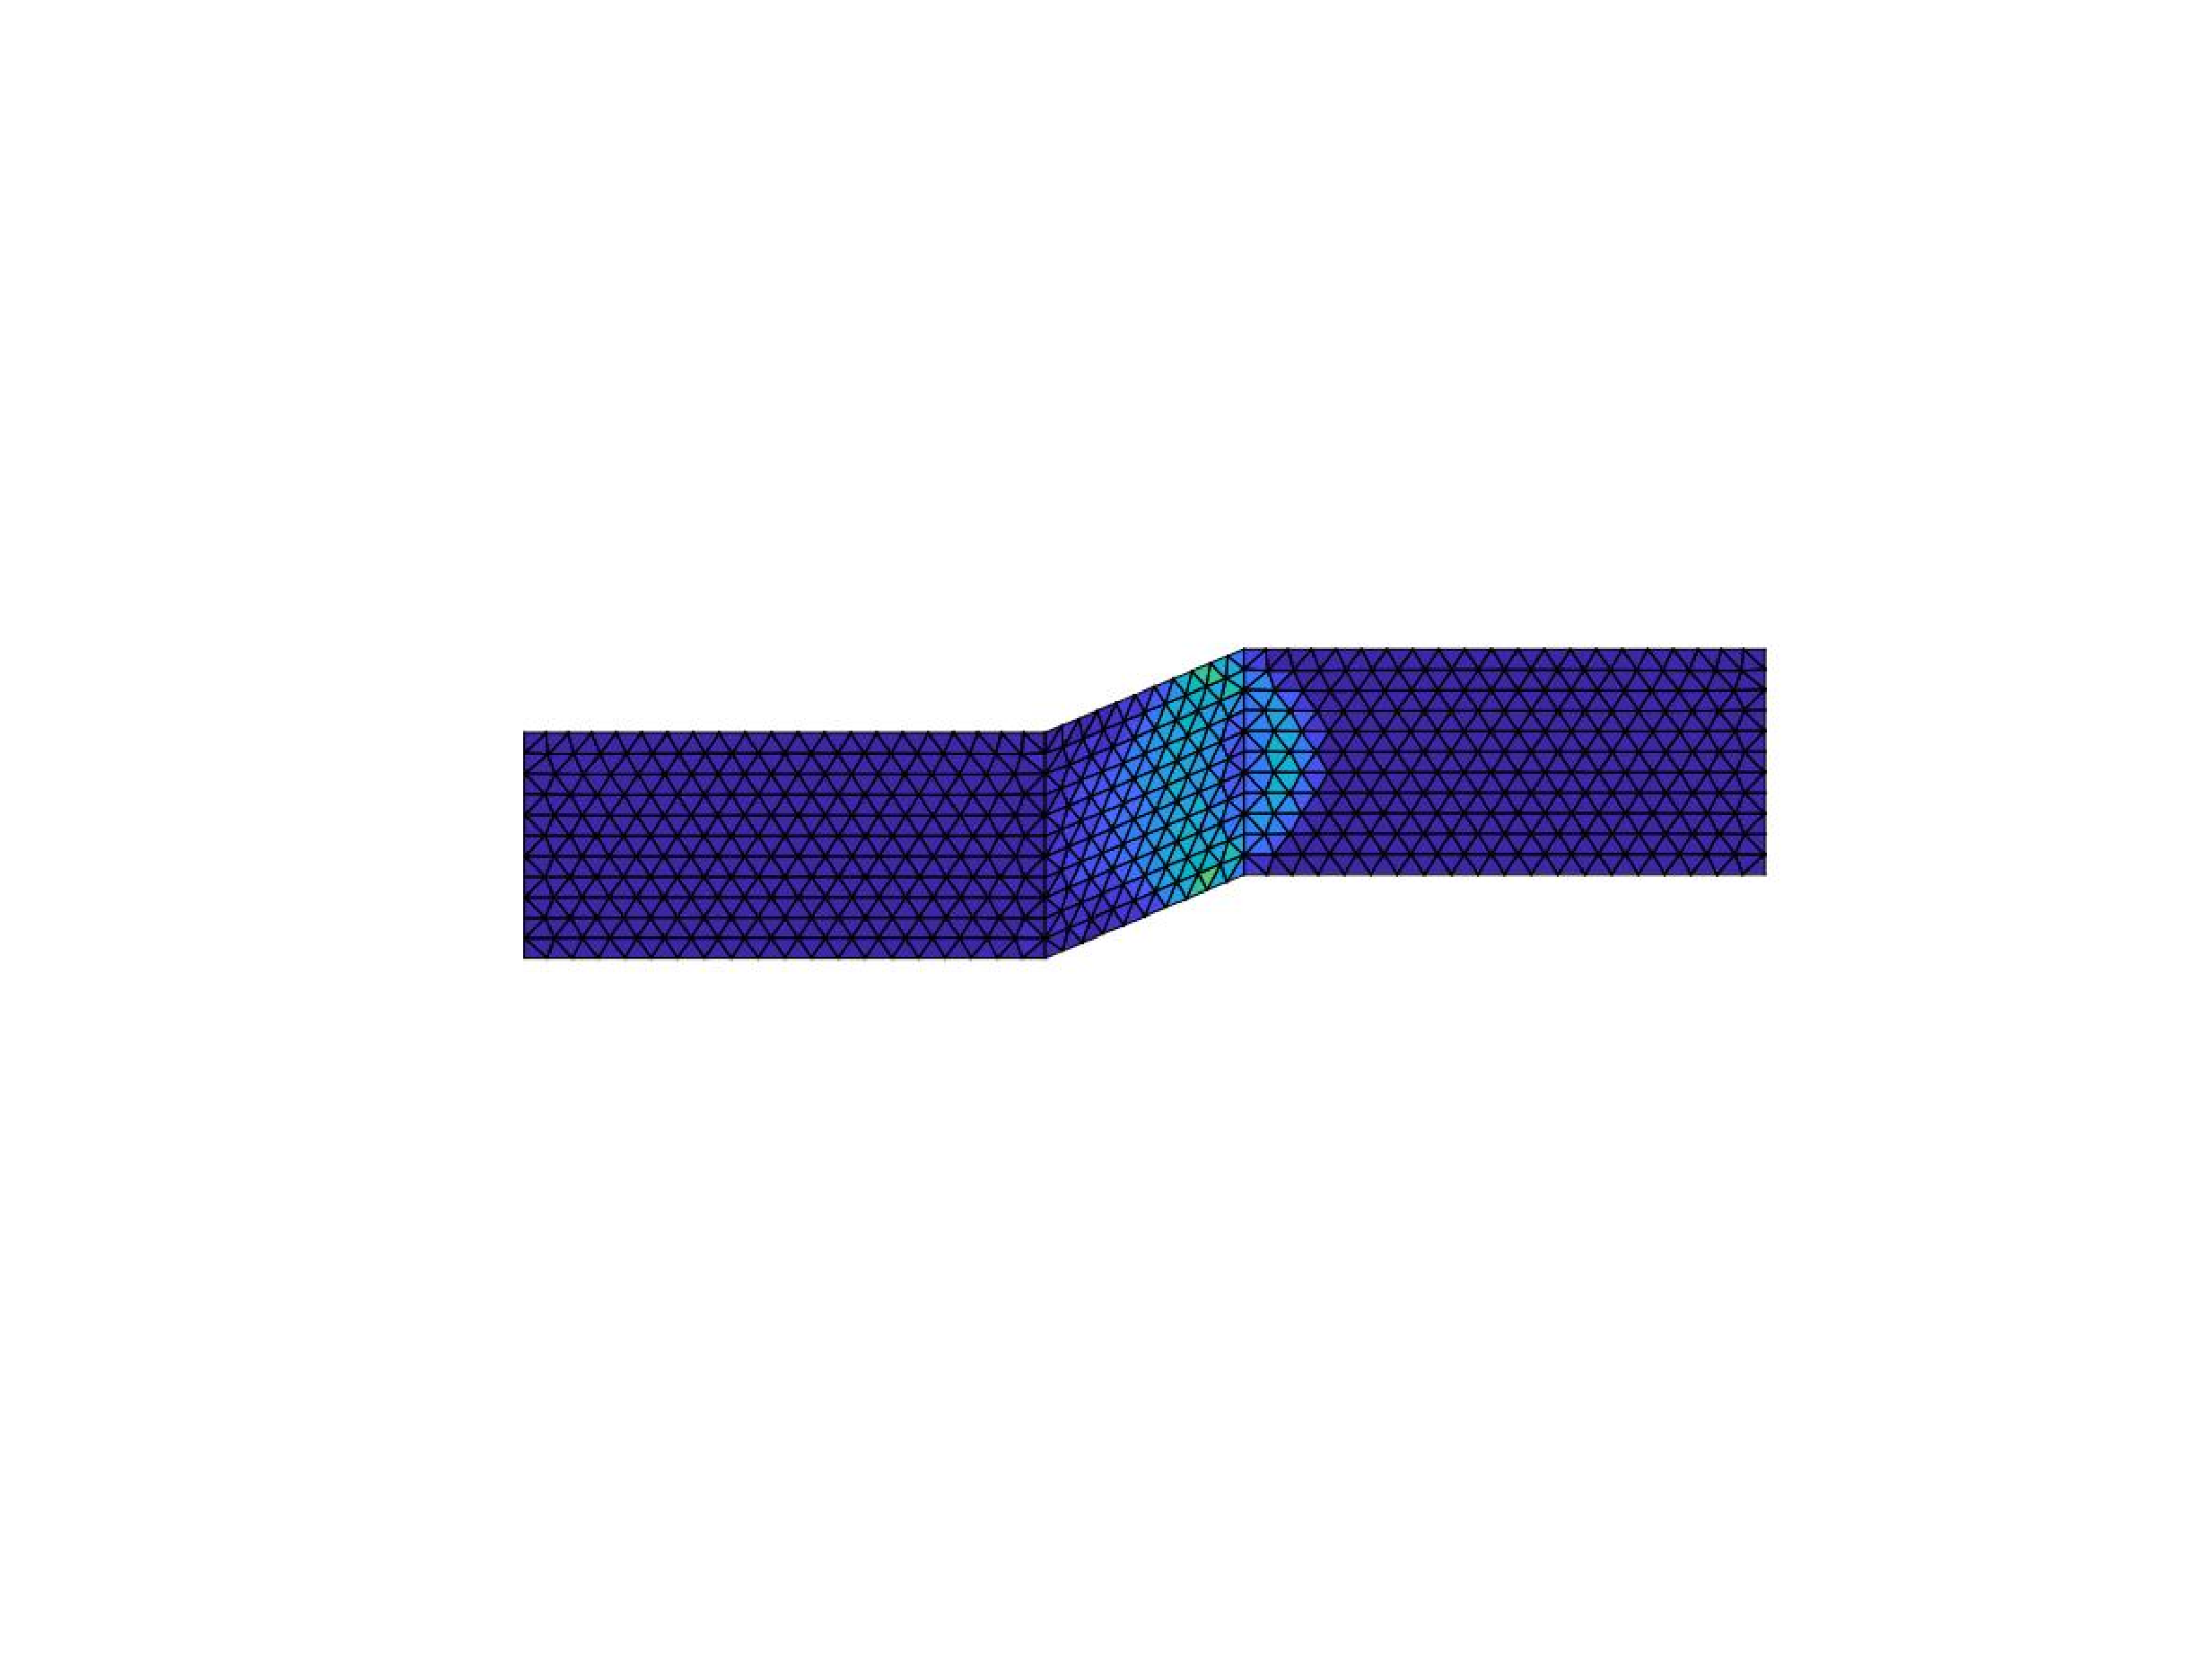
\includegraphics[trim = 100mm 120mm 100mm 120mm,clip=true, width=\linewidth]{img/3Druptuerprocess_step150.eps}
  \end{subfigure}
  \begin{subfigure}[b]{0.45\linewidth}
    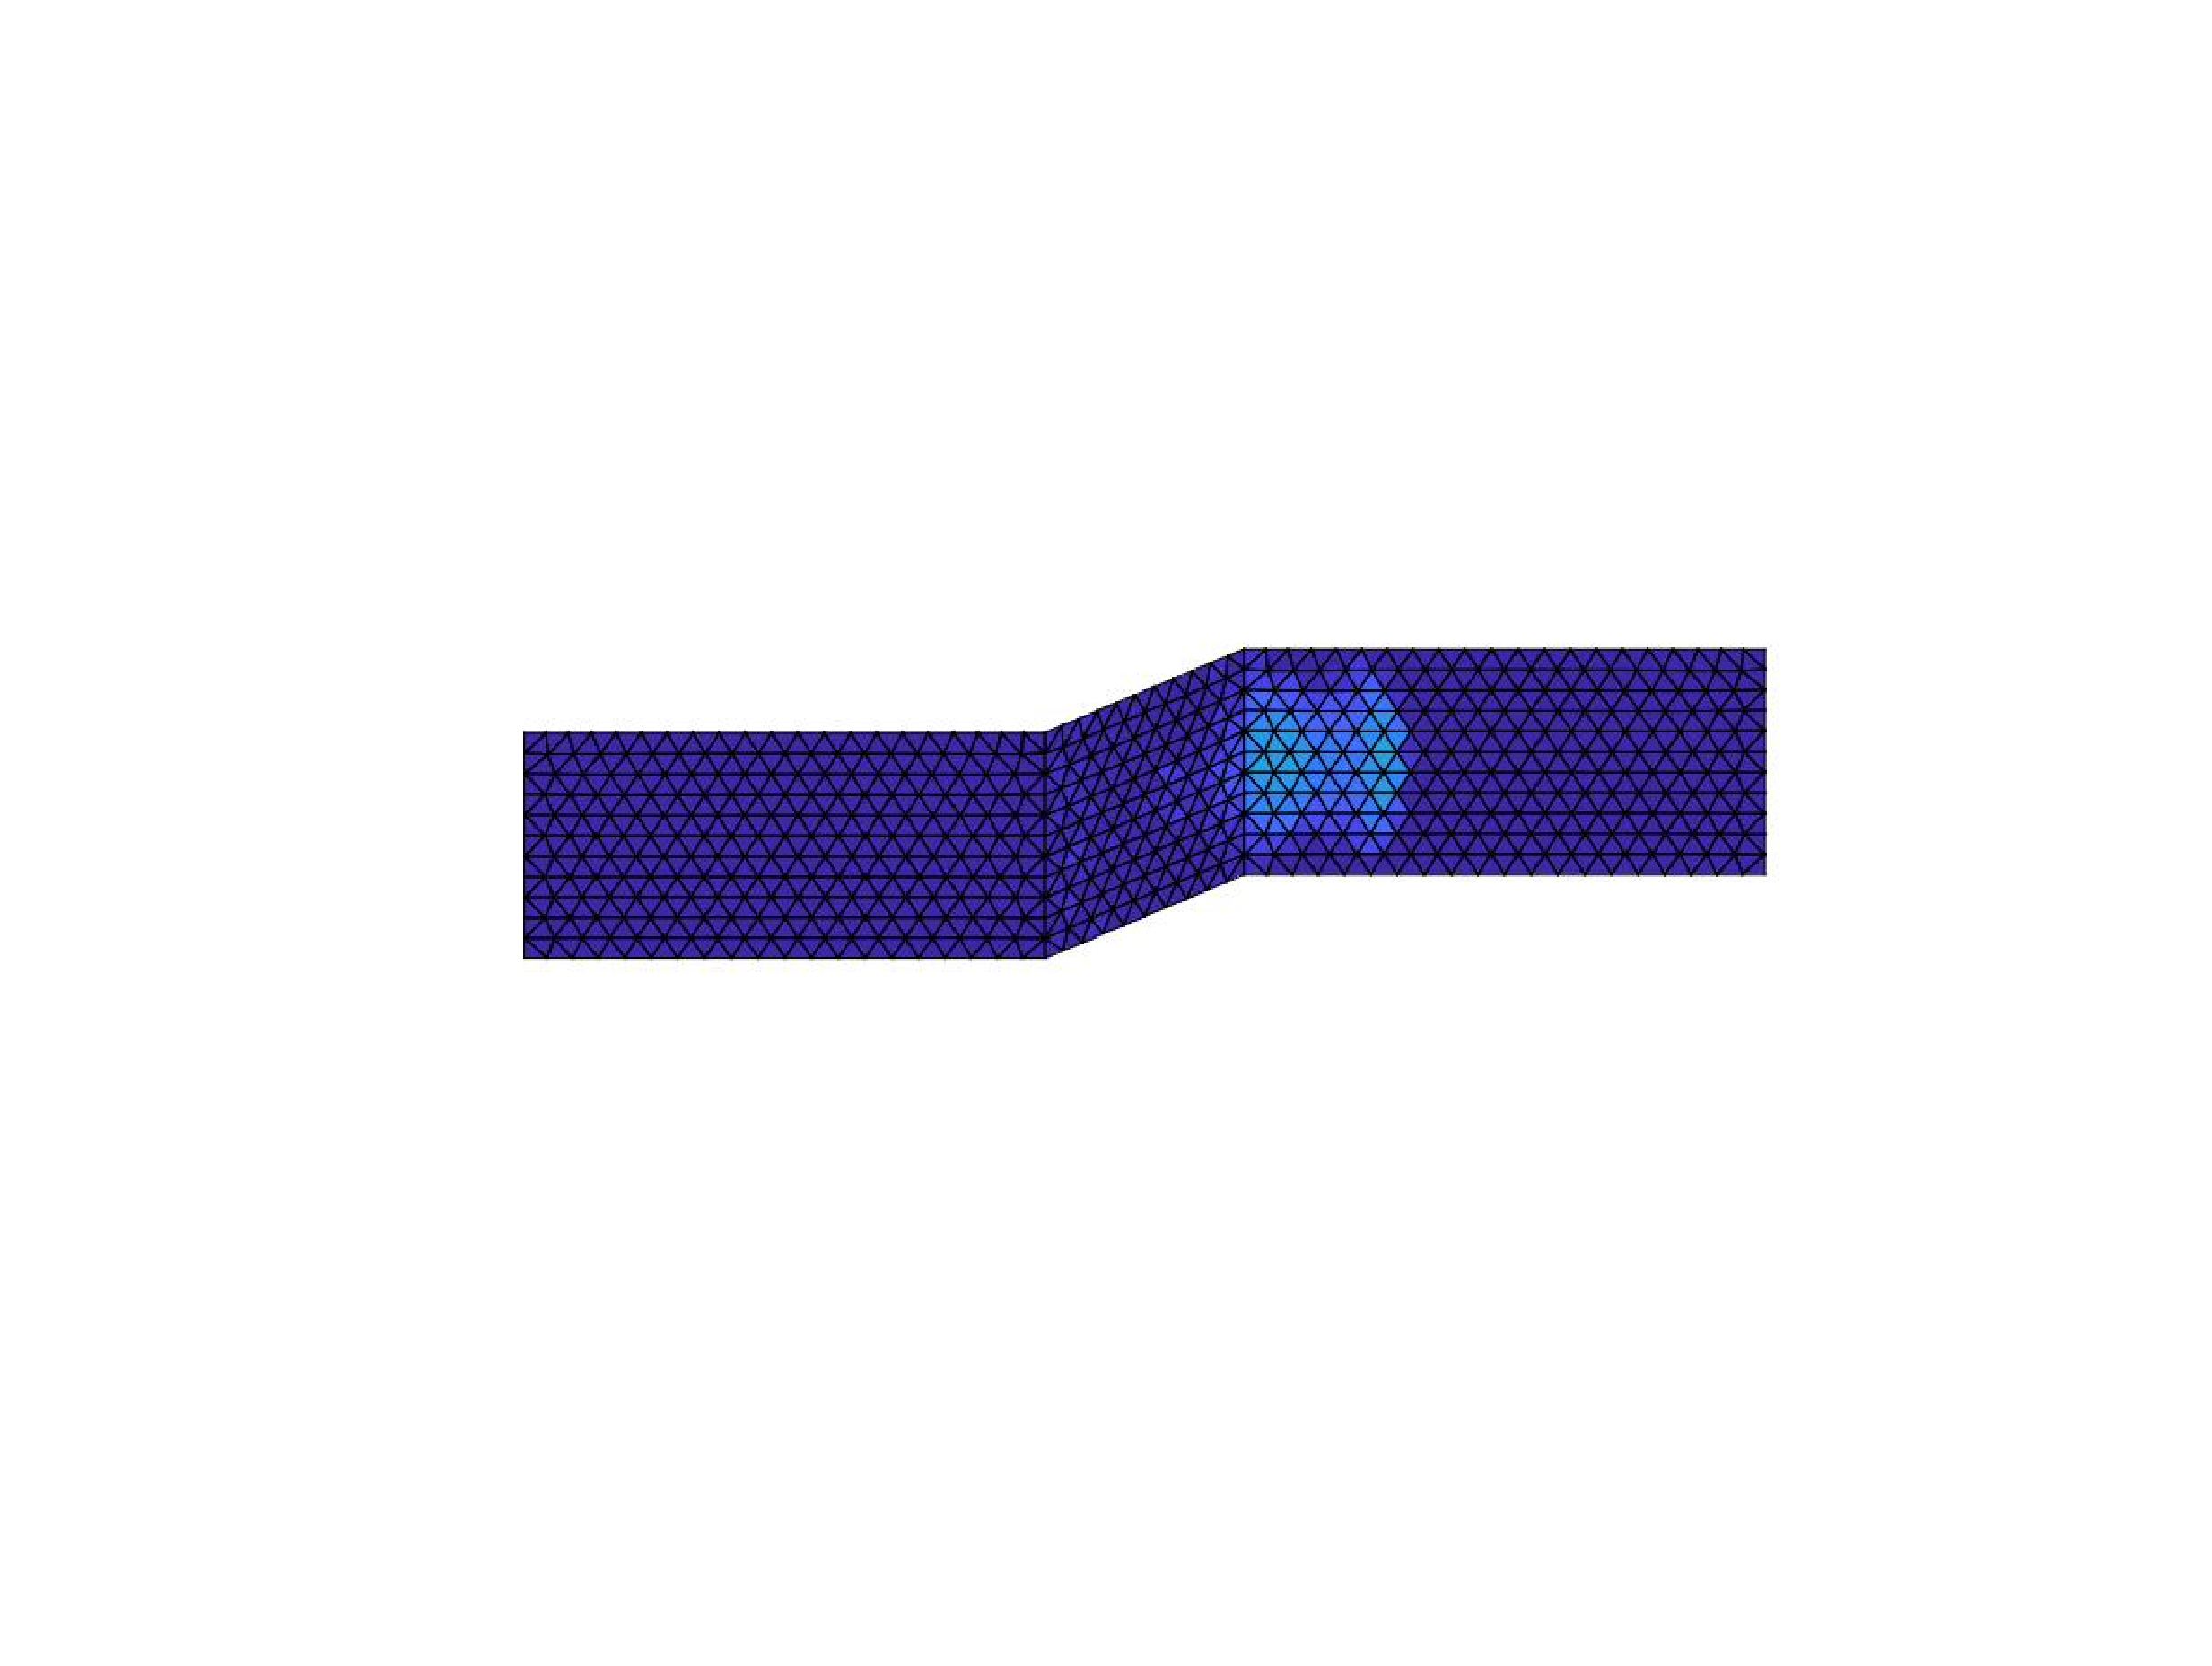
\includegraphics[trim = 100mm 120mm 100mm 120mm,clip=true, width=\linewidth]{img/3Druptuerprocess_step170.eps}
  \end{subfigure}
  \begin{subfigure}[b]{0.45\linewidth}
    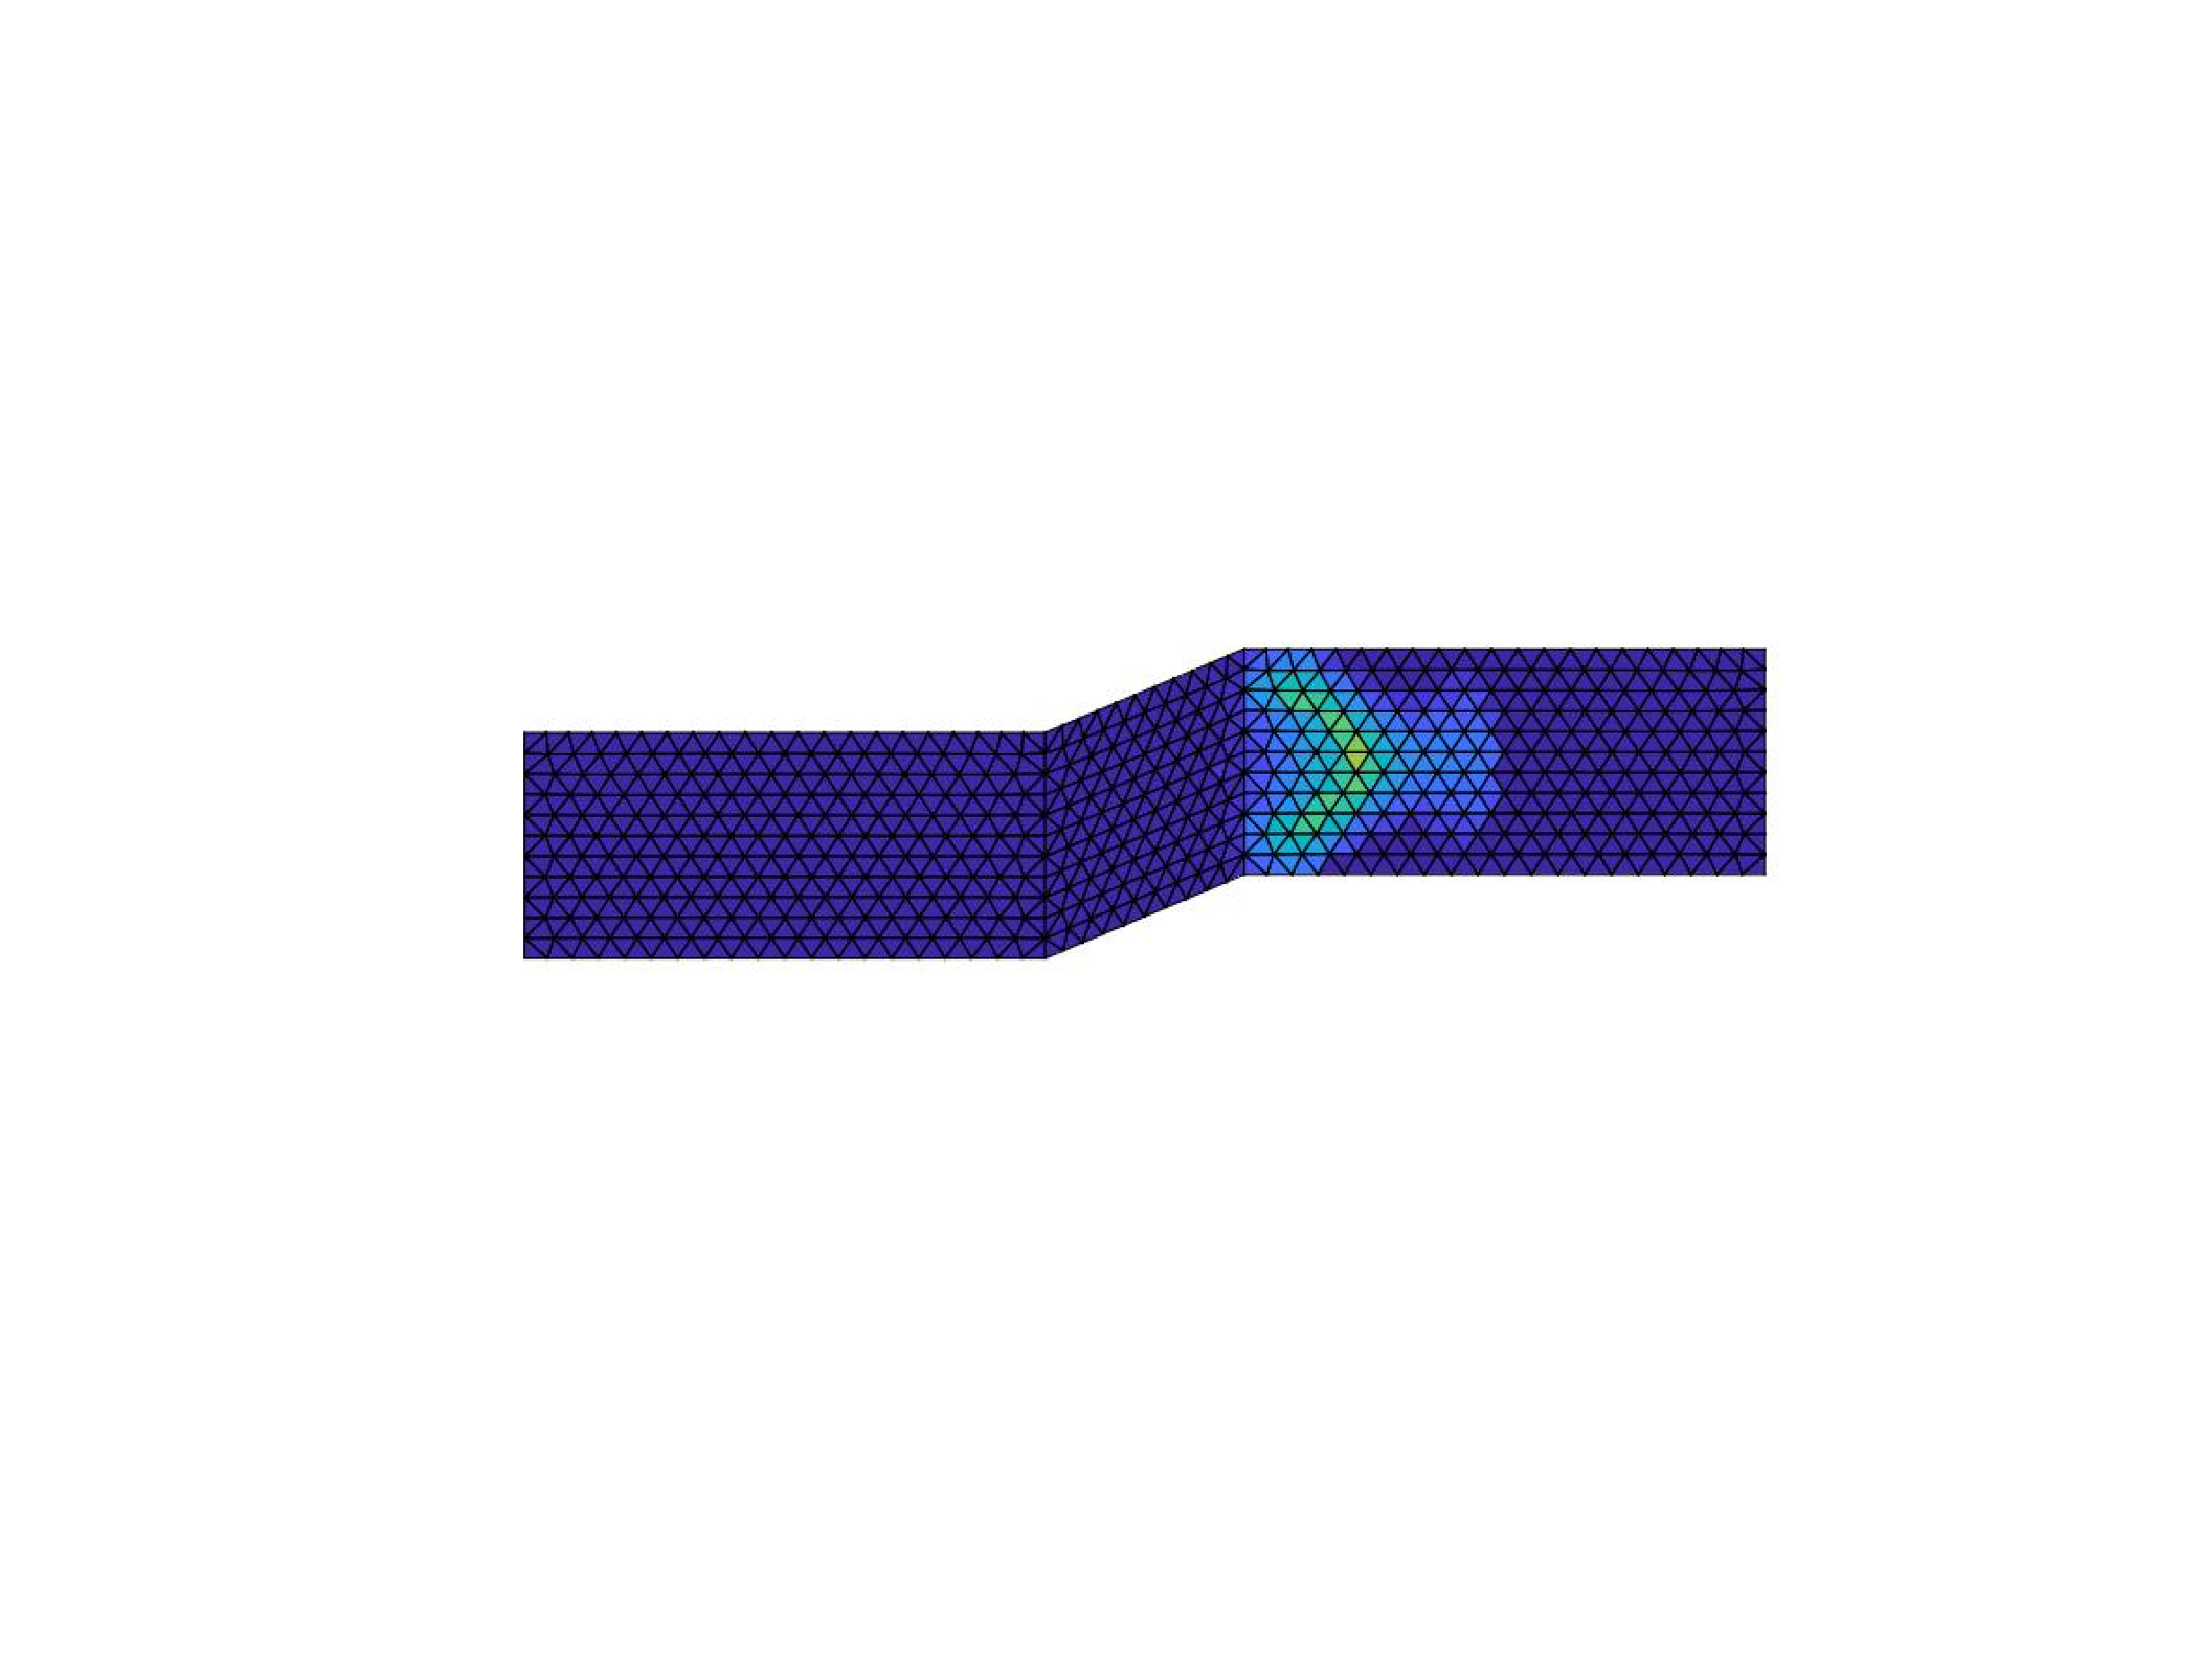
\includegraphics[trim = 100mm 120mm 100mm 120mm,clip=true, width=\linewidth]{img/3Druptuerprocess_step190.eps}
  \end{subfigure}
    \caption{ 弯折断层破裂过程}\label{fig:3d-rupture}
\end{figure}
\end{comment}
	\section{结论分析}
	\indent 在原方法中,积分核计算的时间复杂度为~$O(M^{3}N)$。其中~M~为单元数,N~为时间步。在实际的破裂模拟中,存在许多大尺度即单元数目非常多的模型,若不采取任何加速计算方案将会产生巨大的时间开销。而采用分区计算的加速方案,能够节省~70\%~以上的时间,将大大提高断层破裂过程模拟的效率。

\chapter{总结与展望}
\indent 本文期望实现的目标最终得到了一个不错的结果,即通过分区处理的办法,使得数值模拟破裂过程中积分核值的计算效率得到了显著的提高。我们从~Feng and Zhang(2017)~推导的计算积分核的公式出发,通过到时的不同划分了三个不同区域:初始区,传播区,稳定区。而在初始区和稳定区中,积分核的计算公式得到了相应的简化。通过简化后的表达式我们能快速确定在初始区和稳定区对应的积分核,从而达到了提高计算效率的目的。从本文的分析可以看出,初始区和稳定区的计算占据了积分核计算的绝大部分计算成本。因此对于这两个区域进行加速处理也是很有必要的。一方面我们能以更高的速率获得结果,另一方面可以节约计算资源。而在最后,通过数值算例的验证,既检验了分区计算积分核方法的正确性,另一方面也从实际算例体现了分区法在计算速率上的优越性。\\
\indent 本文虽然对破裂过程中积分核的计算进行极大的优化,但是从分区计算的物理过程我们可以知道,积分核的大部分为0或者稳定值,即在数学上,我们获得的积分核 值为一个三维的稀疏矩阵。而我们在破裂过程的计算中使用了整个矩阵,以为着有大量的0或者稳定值被存入了内存中,造成了内存使用的浪费。因此有必要对于参与破裂过程的积分核矩阵进行一定的压缩处理,以提高内存的利用率。这一部分工作已经展开,详细结果将在附录A中展示。已经实现的情况是,能够对矩阵中所有的~0~元素进行压缩处理。然而又有新的问题产生,为了提高内存的使用率,目前的测量增加了计算的时间的复杂度,也即拿时间换空间。这样的矩阵压缩处理导致了计算效率的降低,与我们最初提升整程序计算效率的初衷相违背。因此,在未来的工作中,如何在增加更小时间复杂的情况下实现对于矩阵的充分压缩是一个需要进一步研究的问题。\\
\indent 无论是对于积分核分区处理达到加速的目的,还是在破裂计算的过程中,压缩矩阵以减小内存的使用,本文的工作都是震源动力学很小的一个方面。但是随着研究的进展,逐渐了解了相关的一些知识,比如网格化分,复杂断层研究等。目前的工作,将为我们进一步学习和研究震源动力学提供一个一窥其究的窗口。





